\documentclass[paper=a4, fontsize=11pt]{scrartcl} %twocolumn, 

\usepackage[utf8]{inputenc} % Use 8-bit encoding that has 256 glyphs

%\usepackage{fourier} % Use the Adobe Utopia font for the document - comment this line to return to the LaTeX default
\usepackage[english]{babel} % English language/hyphenation
\usepackage{amsmath,amsfonts,amsthm, amssymb} % Math packages, use \sim to get tilde

\usepackage{graphicx} % Required for including pictures

\usepackage{booktabs} % Allows the use of \toprule, \midrule and \bottomrule in tables for horizontal lines

%----------Pasting Code---------------

\usepackage{listings} % \usepackage{listings} For inserting code into the document
% Using \usepackage{listingsutf8} for multi-byte encoding of source code

\lstset{breaklines = true, 
numbers = left, 
commentstyle = \color{mygreen}, 
keywordstyle = \color{blue}, 
stringstyle = \color{mymauve},
showstringspaces = true,
basicstyle=\footnotesize
}
%inputencoding = utf8, 
%extendchars = \false

%\usepackage{minted}
\usepackage{color} %for syntax highlighting

\definecolor{mygreen}{rgb}{0,0.6,0}
\definecolor{mygray}{rgb}{0.5,0.5,0.5}
\definecolor{mymauve}{rgb}{0.58,0,0.82}

%------------END--------------

\usepackage{float} %for aligning figures

\usepackage{wrapfig} %for using wraptable or wrapfig

\usepackage{caption}
\usepackage[l2tabu]{nag}

%\usepackage[nottoc]{tocbibind} %to include the bibliography in the contents

\usepackage{verbatim} %use \begin{comment} and \end{comment}. For more complex tasks, check out package:comment

\usepackage{bm} % for printing greek symbols in bold, use \boldsymbol\varepsilon

\usepackage{rotating} % for rotating tables
\usepackage{longtable} % for long tables, 

\usepackage{subcaption} %for supressing table numbering in subtables
\usepackage{makecell} %for multiple lines in a table, enclose the cell value in \thead{A \\ B}

\usepackage{lscape} %for rotating the page with the long table

\usepackage{todonotes} %add TODOs by putting the text in \todo{}

\usepackage{csquotes} %use \begin{displayquotes} to enter a quote

% for changing the nature of urls
%\usepackage[hidelinks]{hyperref} %hides hyperlinks
\usepackage[linktoc = none, linkbordercolor	={0 1 0}]{hyperref}

% custom commands
\newcommand{\mytilde}{\raise.17ex\hbox{$\scriptstyle\mathtt{\sim}$}}

\usepackage{fancyhdr} % Custom headers and footers
\pagestyle{fancyplain} % Makes all pages in the document conform to the custom headers and footers
%\fancyhead{} % No page header - if you want one, create it in the same way as the footers below
\fancyhead[L]{}
\fancyfoot[L]{} % Empty left footer
\fancyfoot[C]{\thepage} % Page numbering for right footer
\fancyfoot[R]{} % Empty right footer
\renewcommand{\headrulewidth}{0pt} % Remove header underlines
\renewcommand{\footrulewidth}{0pt} % Remove footer underlines
\setlength{\headheight}{13.6pt} % Customize the height of the header

\numberwithin{equation}{section} % Number equations within sections (i.e. 1.1, 1.2, 2.1, 2.2 instead of 1, 2, 3, 4)
%\numberwithin{figure}{section} % Number figures within sections (i.e. 1.1, 1.2, 2.1, 2.2 instead of 1, 2, 3, 4)
%\numberwithin{table}{section} % Number tables within sections (i.e. 1.1, 1.2, 2.1, 2.2 instead of 1, 2, 3, 4)

\setlength\parindent{5pt} % Removes all indentation from paragraphs - comment this line for an assignment with lots of text

\graphicspath{{"/home/ad/Desktop/KUL Course Material/SVM (support vector machines)/Exercise Session/images/"}} % Specifies the directory where pictures are stored

%----------------------------------------------------------------------------------------
%	Some Tips For Using This Template
%----------------------------------------------------------------------------------------


\begin{comment}

\end{comment}

%----------------------------------------------------------------------------------------
%	TITLE SECTION
%----------------------------------------------------------------------------------------

\rhead{Akshat Dwivedi}
\lhead{Support Vector Machines}
%\rfoot{\begin{picture}(0,0) \put(-45,-100){\includegraphics[width=3cm]{KU_LeuvenFR}} \end{picture}}
\newcommand{\horrule}[1]{\rule{\linewidth}{#1}} % Create horizontal rule command with 1 argument of height

\title{	
\normalfont \normalsize 
\textsc{\Large KU Leuven} \\ [30pt] % Your university, school and/or department name(s)
\horrule{0.5pt} \\[0.4cm] % Thin top horizontal rule
\huge Support Vector Machines: Final Assingment \\ % The assignment title
\horrule{2pt} \\[0.5cm] % Thick bottom horizontal rule
}

\author{Akshat Dwivedi (Student Number:)\\
\\
Instructor: Prof. Johann Suykens} % Your name

%\date{June 1, 2016} % Today's date or a custom date

\pagenumbering{arabic}

%--------------------------------------------------------------------------------

\begin{document}

\maketitle % Print the title

\thispagestyle{empty}
\clearpage

\tableofcontents
\thispagestyle{empty}
\clearpage
\setcounter{page}{1}

%\listoftodos %makes a list at the top of the document with TODOs

% Begin writing here:

The exercises in this report are for the course Support Vector Machines and are programmed in MATLAB and the report is typeset using \LaTeX.

\section{Exercise Session 1: Classification}

\subsection{Two Gaussians}

A variable X is created as a vector of two sub-variables X$_1$ and X$_2$, where X$_1$ = 1 + $N(0,1)$ and X$_2$ = -1 + $N(0,1)$ and correspondingly, Y = 1 if X$_1$ and -1 otherwise. This results in one predictor (with two classes) and one response (class label). The figure is plotted in figure \ref{1-1}.

\begin{figure}[ht]
\centering
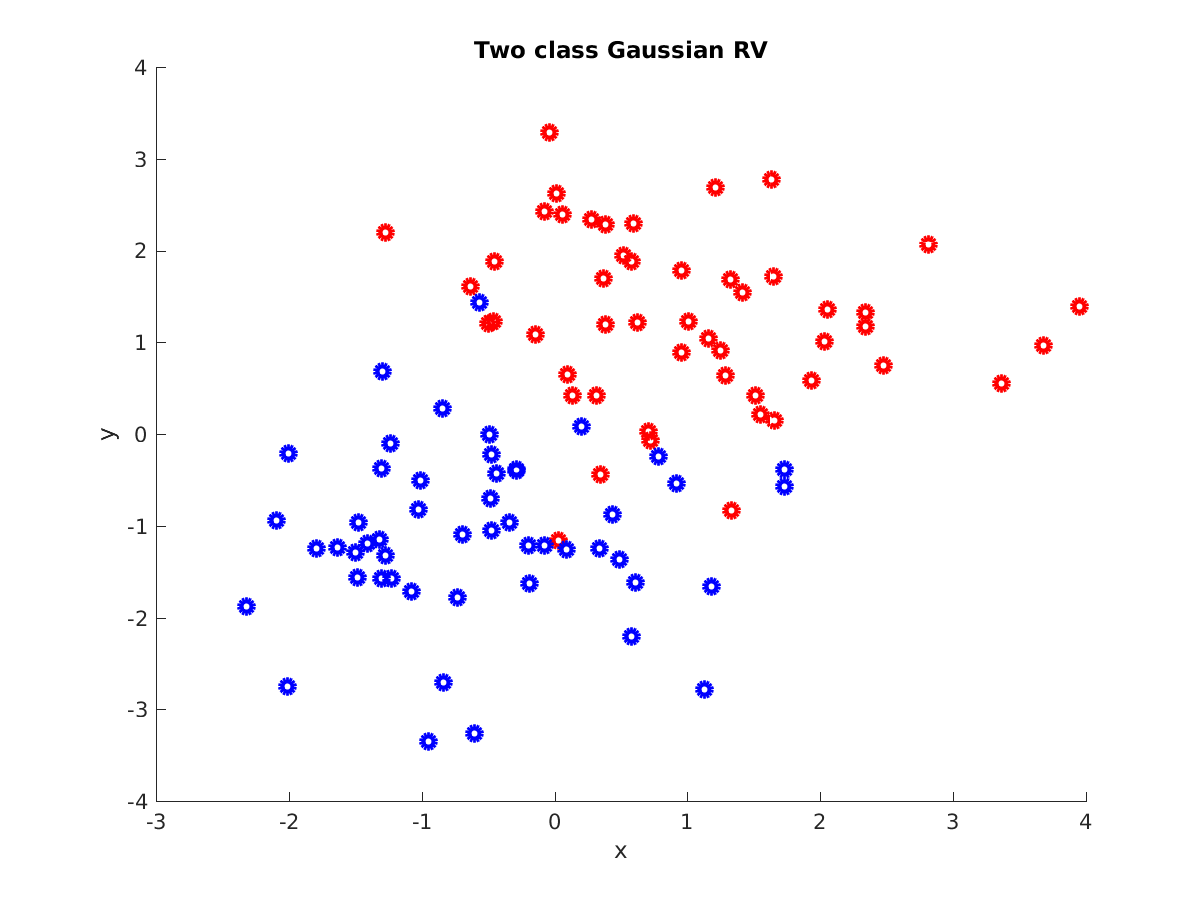
\includegraphics[width = 0.4\textwidth]{plot1-1.png}
\caption{Classification of a two-class variable.}
\label{1-1}
\end{figure}

The two classes here cannot be perfectly separated by a linear hyperplane without misclassifying some of the points in the training set that are overlapping with points from the other class. However, a nonlinear boundary can find a separating hyperplane with lesser misclassified observations. Another approach maybe to use the kernel trick where the inputs are mapped to a higher dimension (a mapping from input space to feature space) where they can be linearly separated by a hyperplane.

\subsection{The Support Vector Machine}

The demo found at \url{http://cs.stanford.edu/people/karpathy/svmjs/demo/} is explored to visually assess the working of an SVM. Each time a data point is added, the linear decision boundary changes to accommodate the addition of that point. Thus, depending on where the point is added (irrespective of class), the change in the decision boundary can be rather drastic. Adding a point on the opposite side of the decision boundary results again in a drastic shift in the decision boundary so as to accommodate this new point and keep the classification cost minimal by finding a new maximum-margin classifier.\\

\begin{figure}[ht]
\centering
	\begin{subfigure}[b]{0.3\textwidth}
		\centering
		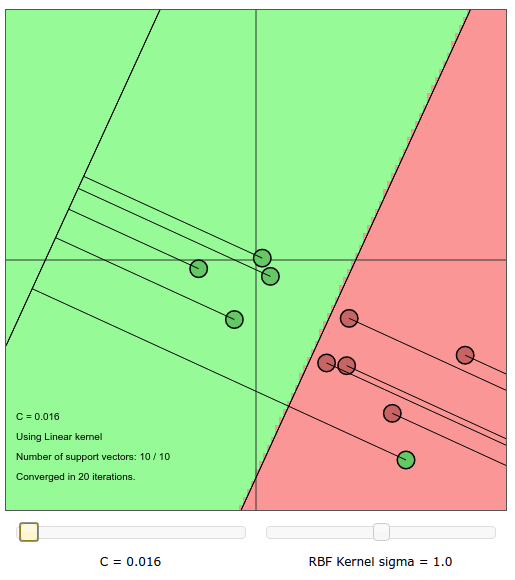
\includegraphics[width = \textwidth]{linear-small-c.png}
		\caption{c = 0.025}
	\end{subfigure}
	\begin{subfigure}[b]{0.3\textwidth}
		\centering
		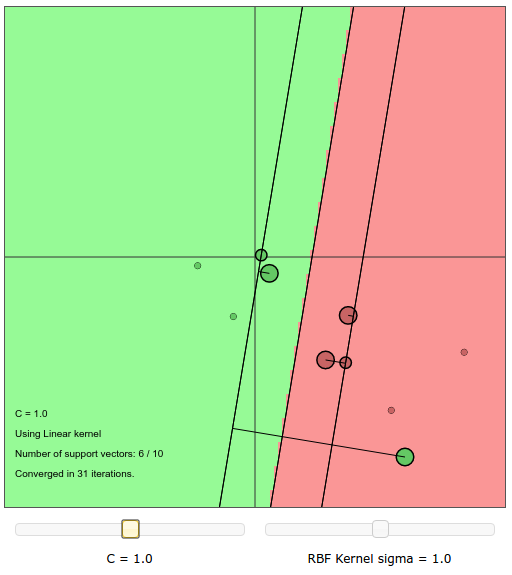
\includegraphics[width = \textwidth]{linear-medium-c.png}
		\caption{c = 1}
	\end{subfigure}
	\begin{subfigure}[b]{0.3\textwidth}
		\centering
		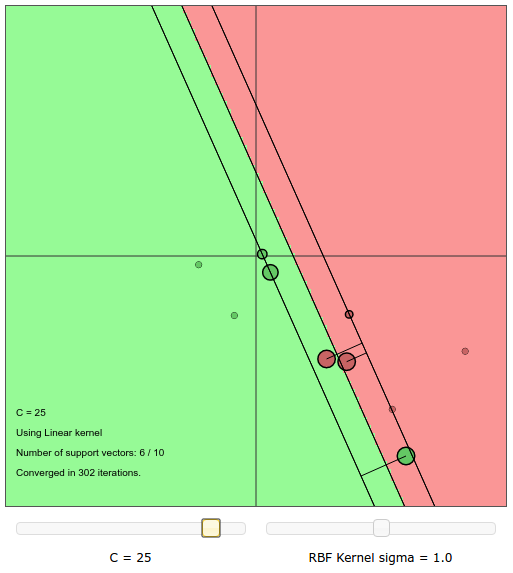
\includegraphics[width = \textwidth]{linear-large-c.png}
		\caption{c = 25}
	\end{subfigure}
\caption{Linear kernel: exploring the role of regularization parameter $c$.}
\label{linear}
\end{figure} 

The parameter $c$ is a regularization parameter that controls the number of points that are used as support vectors. A larger value of $c$ uses less support vectors (indicating more regularization) and a smaller value of $c$ uses a larger fraction of the total points as support vectors (i.e., points closer to the decision boundary). Furthermore, increasing the value of $c$ requires more iterations for the underlying algorithm to converge to the optimal solution. A smaller amount of regularization converges faster.\\

\begin{figure}[ht]
\centering
\begin{subfigure}[b]{0.3\textwidth}
		\centering
		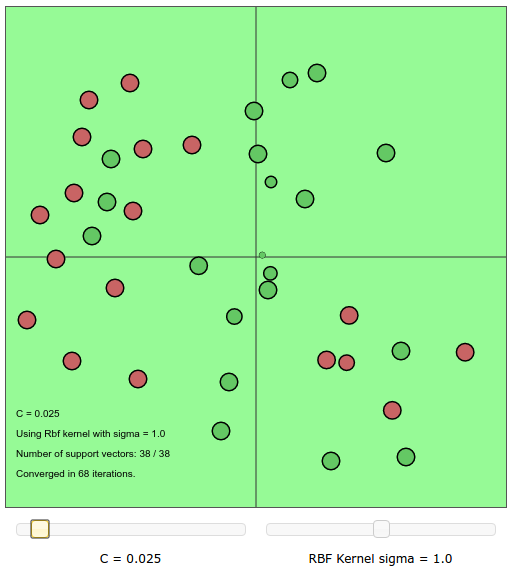
\includegraphics[width = \textwidth]{non-lin-small-c.png}
		\caption{c = 0.025, $\sigma^2$ = 1}
	\end{subfigure}
	\begin{subfigure}[b]{0.3\textwidth}
		\centering
		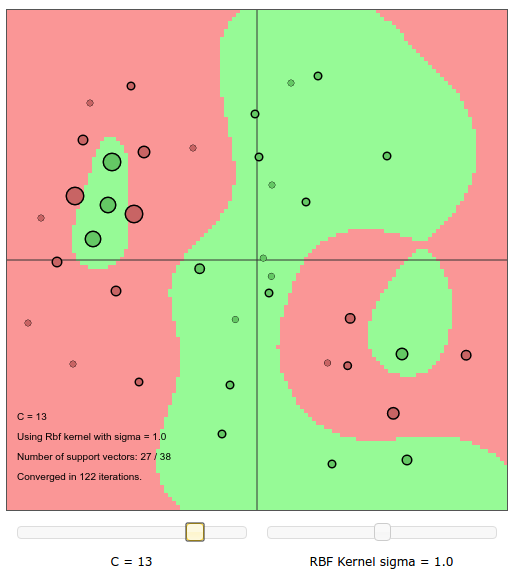
\includegraphics[width = \textwidth]{non-lin-large-c.png}
		\caption{c = 13, $\sigma^2$ = 1}
	\end{subfigure}
	\begin{subfigure}[b]{0.3\textwidth}
		\centering
		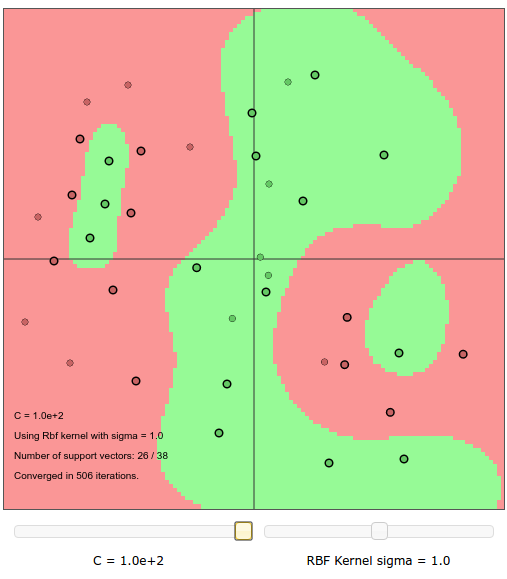
\includegraphics[width = \textwidth]{non-lin-largest-c.png}
		\caption{c = 100, $\sigma^2$ = 1}
	\end{subfigure}
\caption{Non-separable classes. RBF kernel with $\sigma^2$ fixed and c varying.}
\label{non-sep-fixed-sigma}
\end{figure}

Switching back to the RBF kernel from the linear kernel, we see that the classification error decreases drastically and the network is highly adaptive to the addition of new data points irrespective of where the points are added. Furthermore, a much larger fraction of data points are used as support vectors compared to the linear case which is the reason for the low misclassification rate. If the regularization hyperparameter is too small, the whole region is assigned one class label (the dominant class) however increasing this value results in separate regions for the two classes. If two points- one from each class are separated from each other, a small region forms around the points. the important point is that the decision boundary is nonlinear, and hence, is capable of learning from general decision surfaces. The size of the point indicates it's importance in the decision boundary- points which are close to the decision boundary are larger and vice versa. The hyperparameter $\sigma^2$ for the RBF kernel controls the smoothness of the decision boundary. A large $\sigma^2$ value results in a near linear boundary where as a smaller $\sigma^2$ value leads to the decision boundary being more nonlinear (rough).

\begin{figure}[ht]
\centering
\begin{subfigure}[b]{0.3\textwidth}
		\centering
		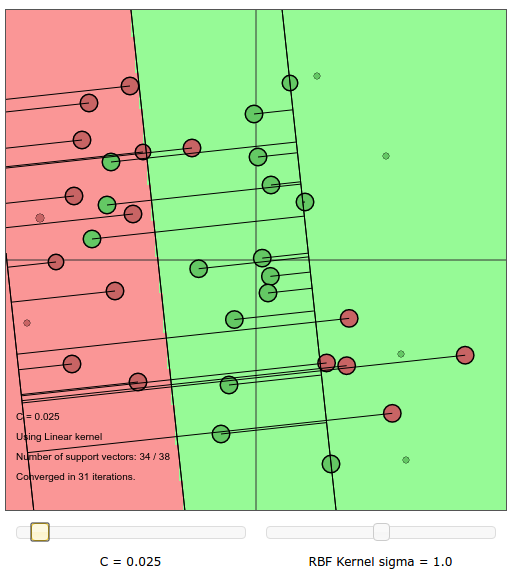
\includegraphics[width = \textwidth]{non-sep-lin-small-c.png}
		\caption{c = 0.025}
	\end{subfigure}
	\begin{subfigure}[b]{0.3\textwidth}
		\centering
		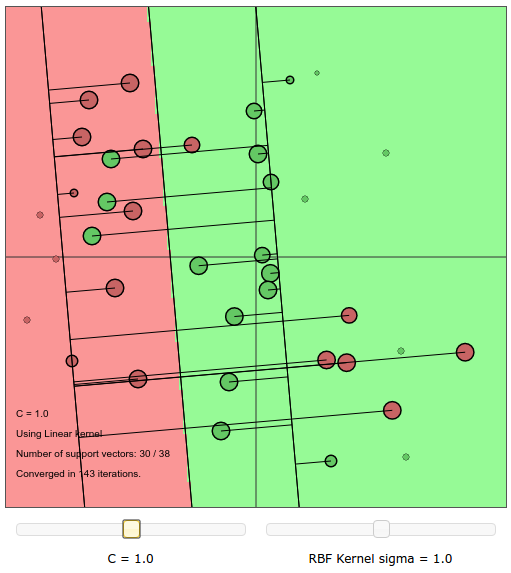
\includegraphics[width = \textwidth]{non-sep-lin.png}
		\caption{c = 1}
	\end{subfigure}
	\begin{subfigure}[b]{0.3\textwidth}
		\centering
		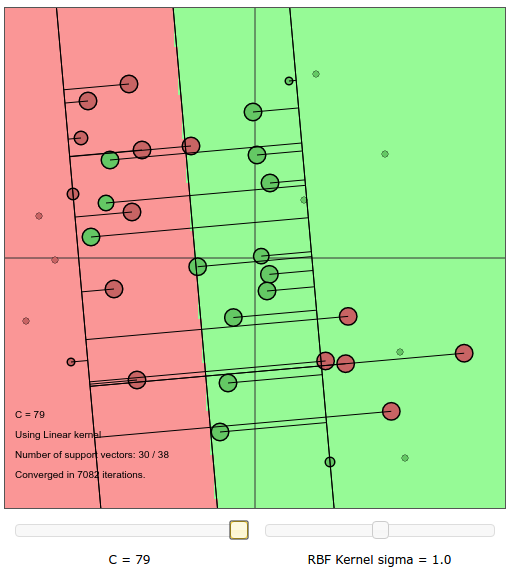
\includegraphics[width = \textwidth]{non-sep-lin-large-c.png}
		\caption{c = 79}
	\end{subfigure}
\caption{Non-separable classes and linear kernel.}
\label{non-sep-linear}
\end{figure}

% part 5
We create a dataset with overlapping regions (thus the two classes are not linearly separable). This is shown in figure \ref{non-sep-fixed-c}(a). If a linear kernel is used, about half the points are used as support vectors, as compared to the RBF kernel where nearly all the points are used as support vectors. However, the misclassification in case of linear kernel is much higher where as it is nearly zero in case of the RBF kernel. In case of RBF kernel, a small amount of $\sigma$ value keeps the size of the Gaussian kernel at the support vectors small.\\

\begin{figure}[ht]
\centering
\begin{subfigure}[b]{0.3\textwidth}
		\centering
		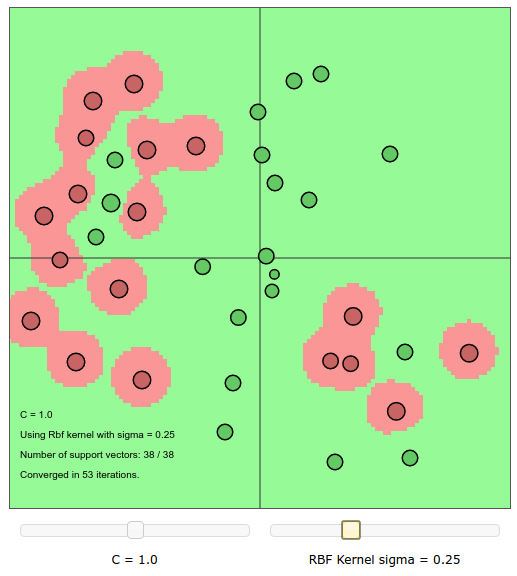
\includegraphics[width = 1.1\textwidth]{non-lin-small-sigma.png}
		\caption{c = 1, $\sigma^2$ = 0.25}
	\end{subfigure}
	\begin{subfigure}[b]{0.3\textwidth}
		\centering
		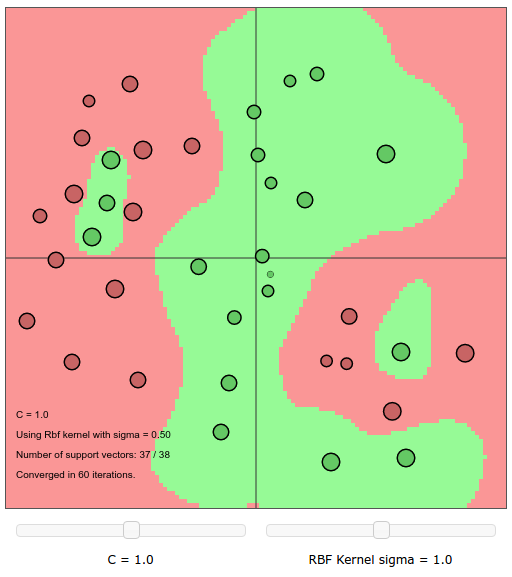
\includegraphics[width = 1.1\textwidth]{non-lin.png}
		\caption{c = 1, $\sigma^2$ = 1}
	\end{subfigure}
	\begin{subfigure}[b]{0.3\textwidth}
		\centering
		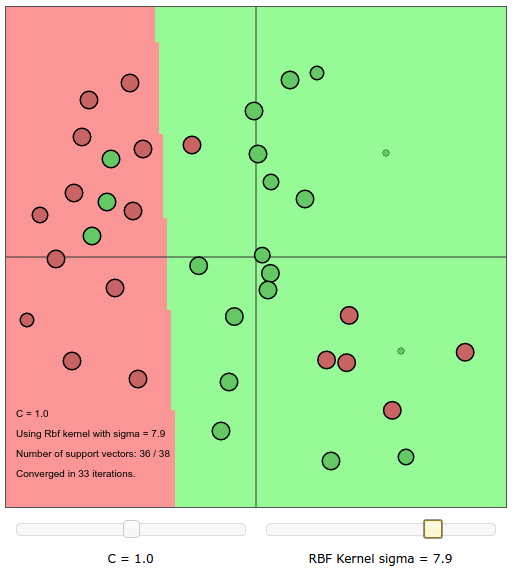
\includegraphics[width = 1.1\textwidth]{non-lin-large-sigma.png}
		\caption{c = 1, $\sigma^2$ = 8}
	\end{subfigure}
\caption{Non-separable classes with RBF kernel and fixed c.}
\label{non-sep-fixed-c}
\end{figure} 

The importance of the support vector changes as each new point is added to the dataset or if the hyperparameter values are tweaked. A data point becomes a support vector if it happens to be close to the decision boundary. If a new point is added to class A region that is from class B then this new point will become a support vector due to the corresponding slack variable becoming active in the optimization process.

\subsection{Using LS-SVMlab}

\subsubsection{Demo}

The demo shows how to use the toolbox for classification. Input matrix is generated as a 30 x 2 matrix $\mathbf{M}$ with $m_{ij} \sim N(0,1)$ entries and the final input matrix $\mathbf{X}$ is created with each entry $x_{ij} = 2 m_{ij} - 1$. The response variable $\mathbf{Y}$ is created as $\mathbf{Y} = \text{sign\{sin}(\textbf{X}_1 + \textbf{X}_2)\}$. The regularization ($\gamma$) parameter is chosen to be 10 which selects the trade-off between fitting-error minimization and smoothness. In case of the RBF kernel, $\sigma^2$ is the bandwidth (hyper-)parameter and is taken to be 0.2. The model is trained on the training set and can be evaluated on new data points by using the command \texttt{simlssvm} and the result for 2 features can be plotted and examined visually as is done in figure \ref{svm-demo}. \texttt{prelssvm} is used to preprocess the input data before training the model. Continuous predictors are scaled to have zero mean and unit variance; binary variables are rescaled to \{-1,+1\} and categorical predictors are left untouched. 

\begin{figure}[ht]
\centering
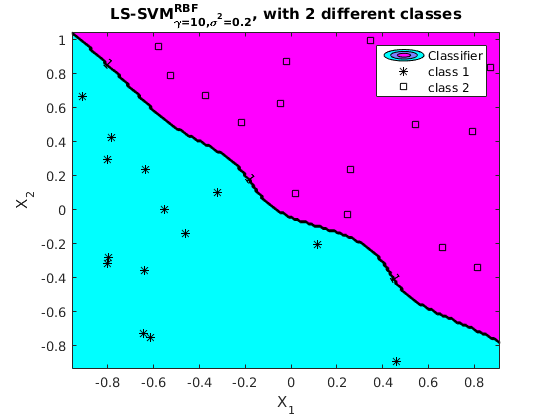
\includegraphics[width = 0.6\textwidth]{lssvm-demo.png}
\caption{LS-SVM demo: two class classification of a system with 2 features. The decision boundary using an RBF kernel is shown as a solid black line.}
\label{svm-demo}
\end{figure}

\subsubsection{Iris dataset}

In this section, the classic Iris dataset is used for classification and different kernels (linear, polynomial, RBF) are explored. The dataset is divided into 100 points in the training set and 20 points in the test set. First, a linear LS-SVM is fit to the training set. The decision boundary is plotted in figure \ref{iris-poly}(a). Number of misclassified observations are 11/20 ($\approx$ 55\%). Next a polynomial kernel is tried with degree 2 (quadratic kernel) and 5. Note: a polynomial kernel with degree 1 is simply a linear kernel. These are plotted in figure \ref{iris-poly}. It is observed that for degree $\geq 3$ the error rate drops to zero with the error rate at degree = 2 equalling 5\%. The polynomial kernel is formulated as $K(x,y) = (x^T y + c)^d$ where $d$ denotes the degree of the polynomial. In the middle figure, we see the decision boundary is quadratic which is to be expected from a quadratic polynomial kernel. In case of degree 5, the kernel seems to be fitting erratically towards the edges of the feature space where there are no data points. 

\begin{figure}[ht]
\centering
	\begin{subfigure}[b]{0.3\textwidth}
		\centering
		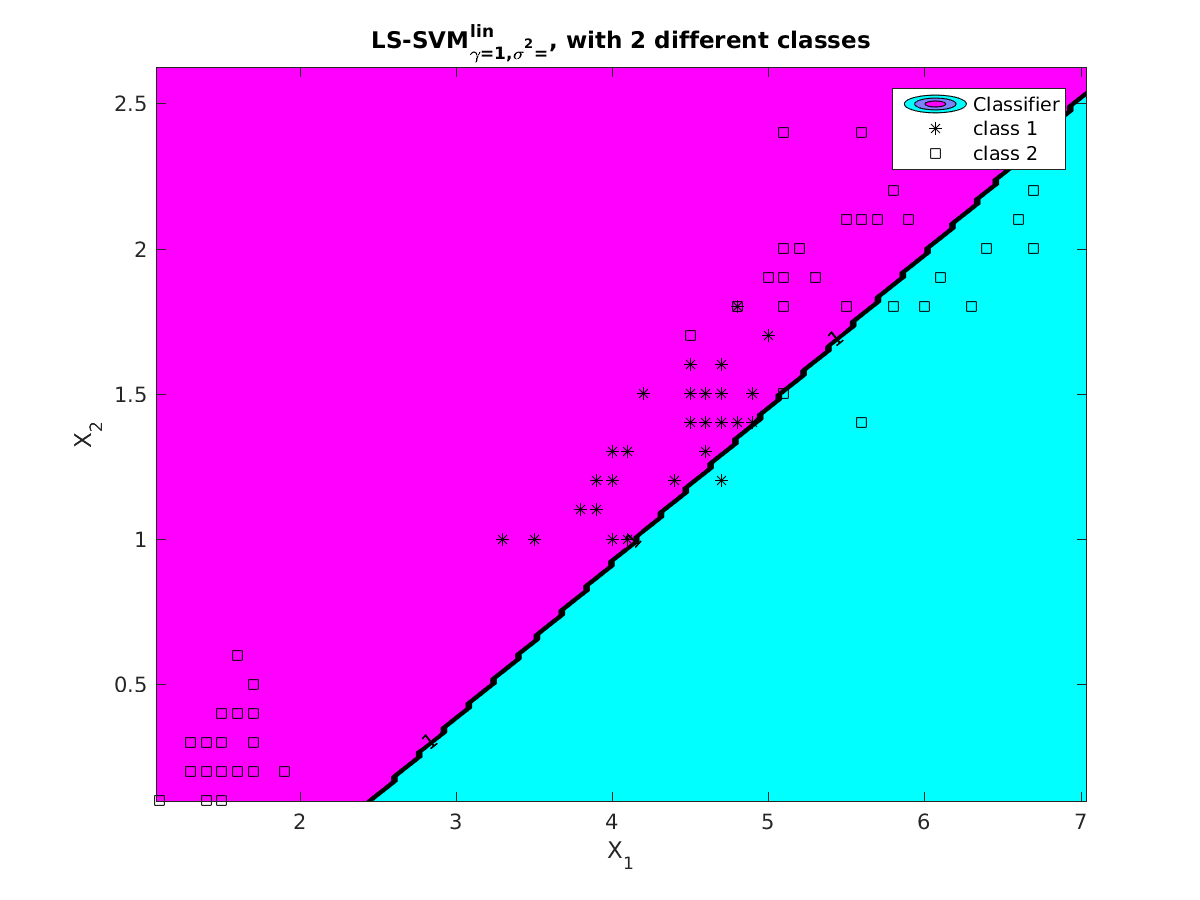
\includegraphics[width = \textwidth]{iris-linear.png}
		\caption{$n_{miss} = 11$, err rate: 55\%}
	\end{subfigure}
	\begin{subfigure}[b]{0.3\textwidth}
		\centering
		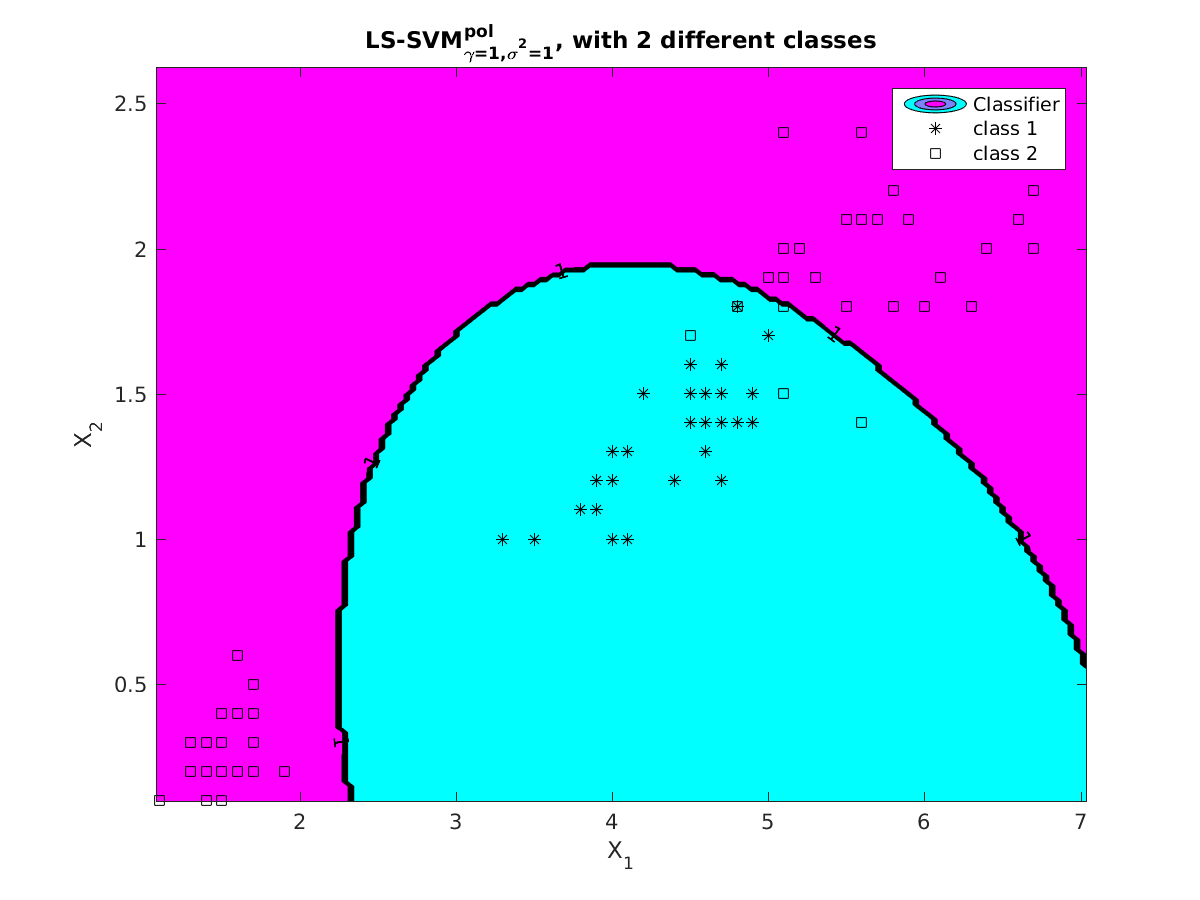
\includegraphics[width = \textwidth]{iris-poly-2.png}
		\caption{$n_{miss} = 1$, err rate: 5\%}
	\end{subfigure}
	\begin{subfigure}[b]{0.3\textwidth}
		\centering
		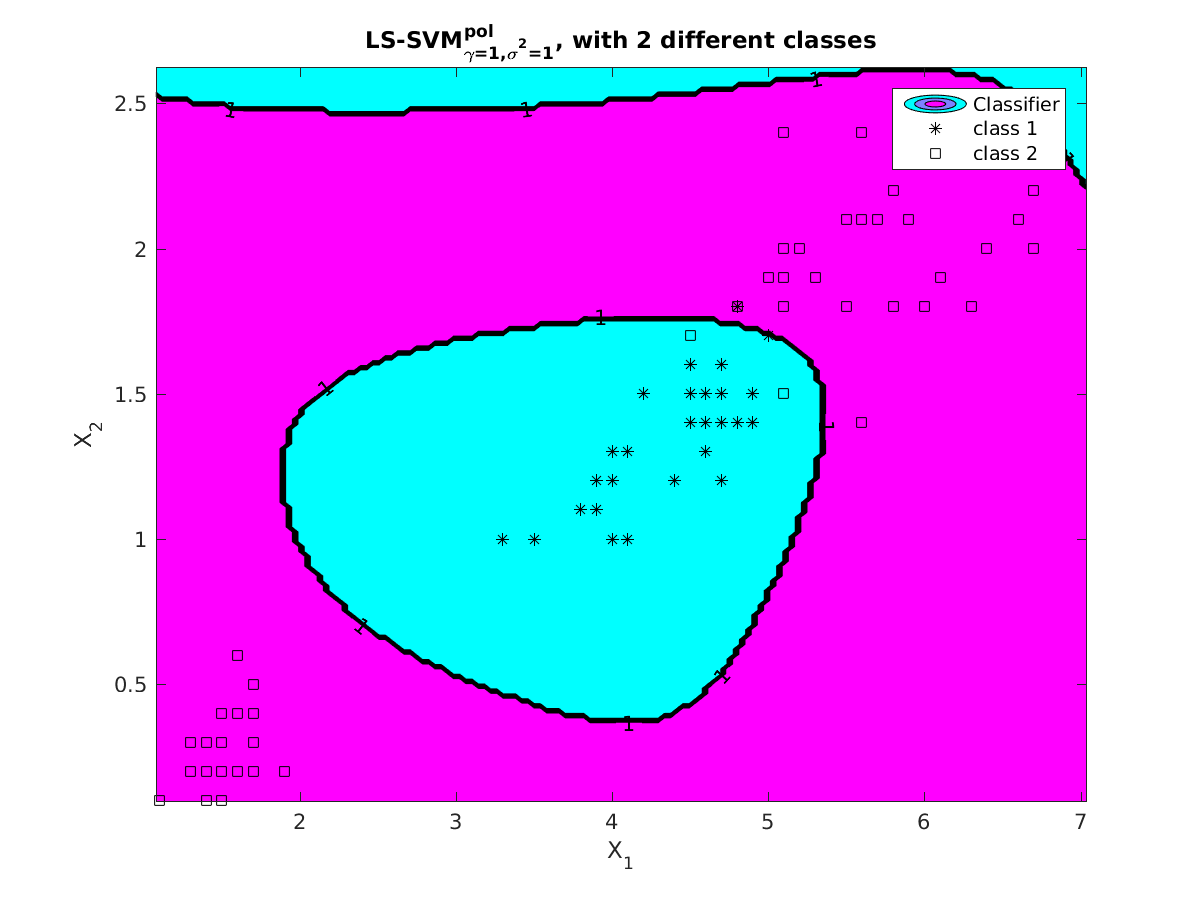
\includegraphics[width = \textwidth]{iris-poly-5.png}
		\caption{$n_{miss} = 0$, err rate:  0\%}
	\end{subfigure}
\caption{Iris classification: Linear kernel (a), polynomial kernel of degree 2 (b), and polynomial kernel of degree 5 (c). The misclassification percentages are reported on the test set. The error rate drops to zero for degree $\geq$ 3.}
\label{iris-poly}
\end{figure} 

For the RBF kernel case, we keep the regularization parameter ($\gamma$) fixed at 1 and vary the values of the RBF kernel parameter ($\sigma^2 \in \{0.01, 0.1, 1, 5, 10, 25\}$). The error rate for the first value (0.01) is 10\% (2 misclassified observations) after which the error rate drops to zero except for the last $\sigma^2$ value (25) at which point the uncertainty is too large and all points are assigned to one out of the two classes (which results in 50\% error rate on the test set). This is plotted in figure \ref{iris-rbf}.\\

\begin{figure}[ht]
\centering
	\begin{subfigure}[b]{0.3\textwidth}
		\centering
		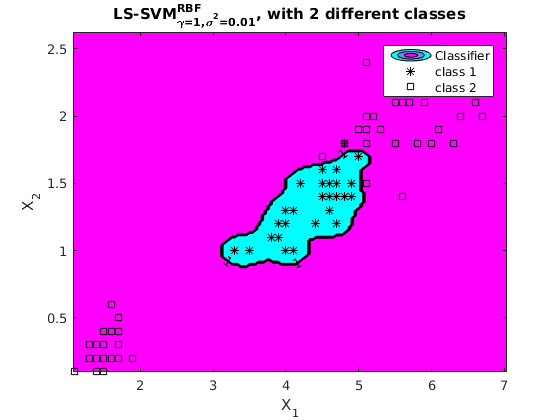
\includegraphics[width = \textwidth]{iris-rbf-0-01.png}
		\caption{$\sigma^2 = 0.01$}
	\end{subfigure}
	\begin{subfigure}[b]{0.3\textwidth}
		\centering
		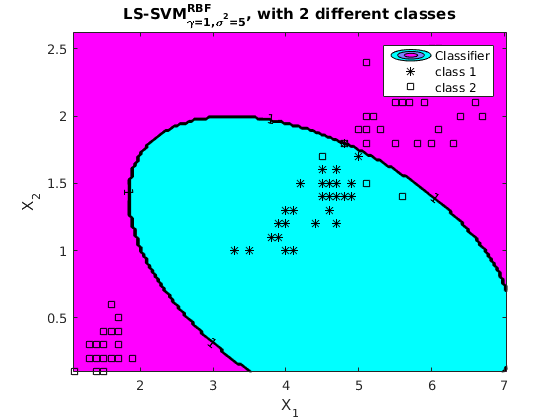
\includegraphics[width = \textwidth]{iris-rbf-5.png}
		\caption{$\sigma^2 = 5$}
	\end{subfigure}
	\begin{subfigure}[b]{0.3\textwidth}
		\centering
		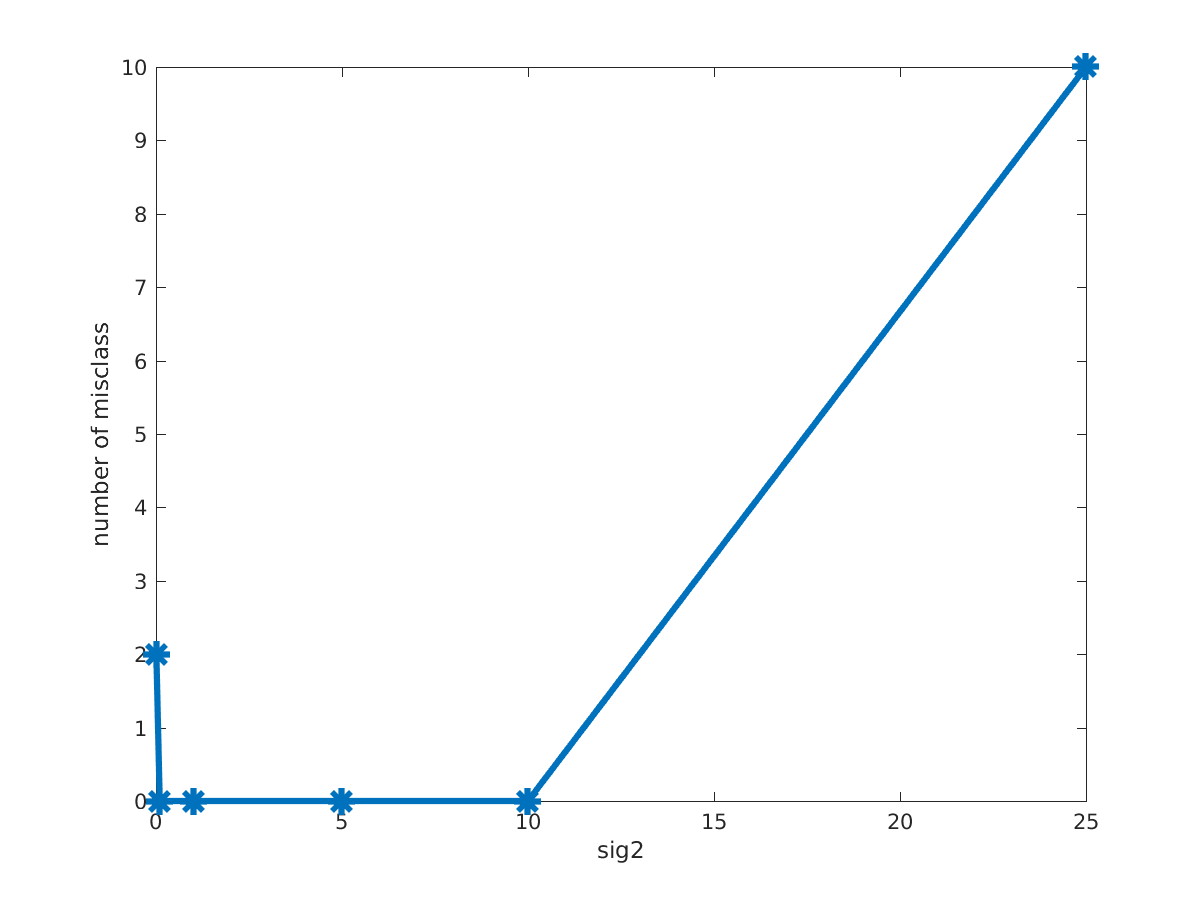
\includegraphics[width = \textwidth]{iris-rbf-sigma-rate.png}
		\caption{$n_{misclass}$ vs $\sigma^2$}
	\end{subfigure}
\caption{Iris classification: RBF kernel with different values for the hyperparameter $\sigma^2$ set to 0.01 (a), 5 (b) and the plot of $n_{misclass}$ as a function of $\sigma^2$ on the test set.}
\label{iris-rbf}
\end{figure}

From this figure, we see that for small $\sigma^2$, the class region is quite small which leads to non-zero error rate on the test set. However, as $\sigma^2$ increases, the uncertainty around the separating margin increases leading to larger regions for each of the classes. Thus, this leads to a reduction in the error rate of the classifier. Figure \ref{iris-rbf}(c) shows the number of misclassified cases on the test set as a function of the hyperparameter $\sigma^2$. Next, we do the same with the regularization parameter $\gamma$ ($\in \{0.01, 0.1, 1, 5, 10, 15, 25\}$) while holding $\sigma^2 = 1$ fixed and the results are shown in figure \ref{iris-rbf-gam}.\\

\begin{figure}[ht]
\centering
	\begin{subfigure}[b]{0.3\textwidth}
		\centering
		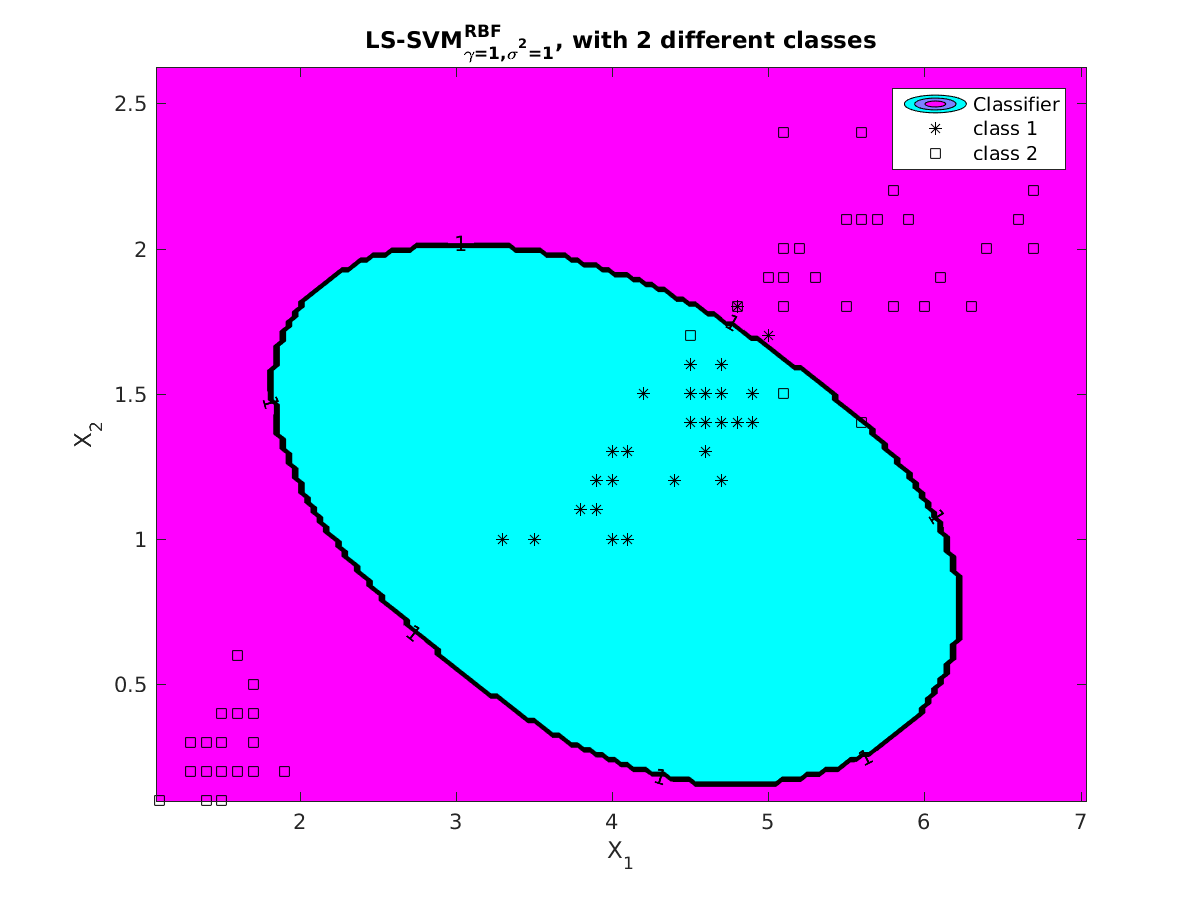
\includegraphics[width = \textwidth]{iris-rbf-gam-1.png}
		\caption{$\gamma = 5$}
	\end{subfigure}
	\begin{subfigure}[b]{0.3\textwidth}
		\centering
		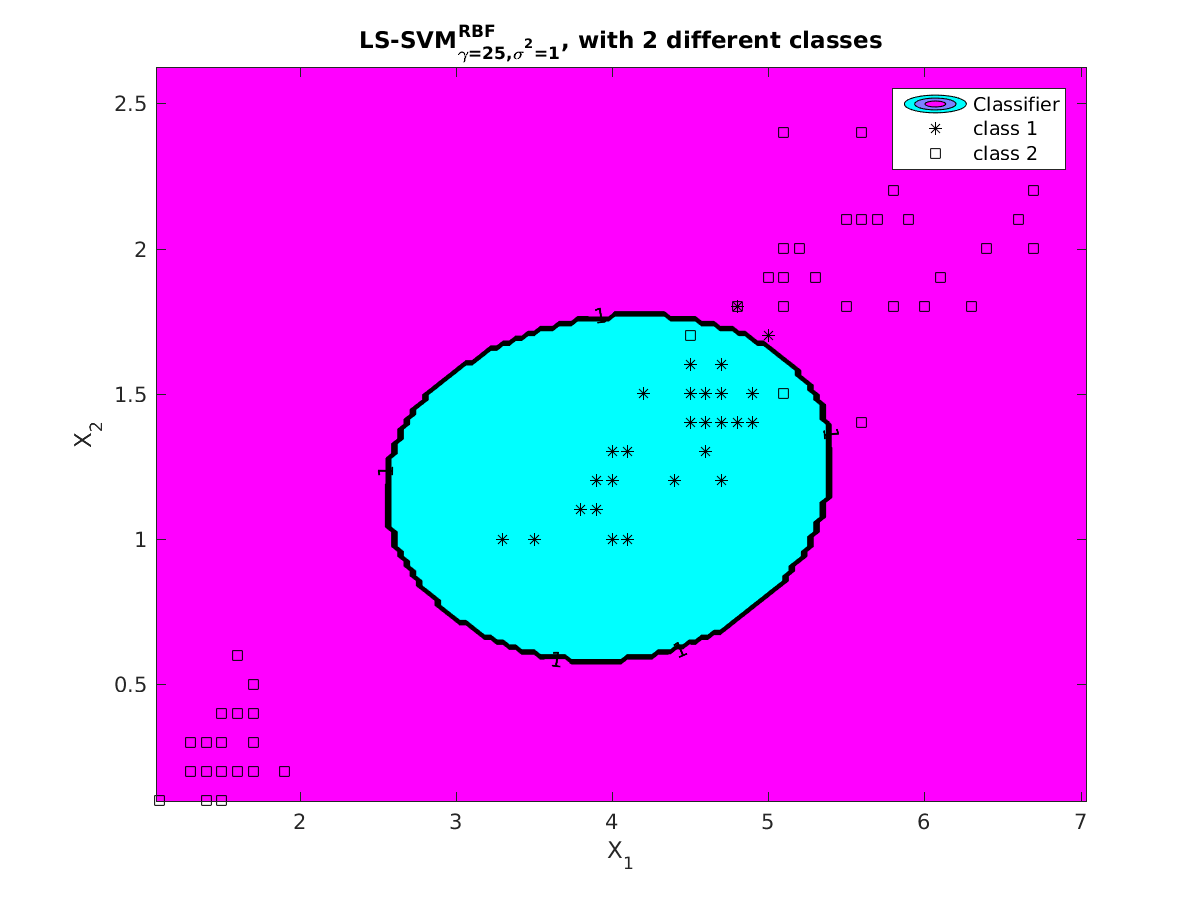
\includegraphics[width = \textwidth]{iris-rbf-gam-25.png}
		\caption{$\gamma = 25$}
	\end{subfigure}
	\begin{subfigure}[b]{0.3\textwidth}
		\centering
		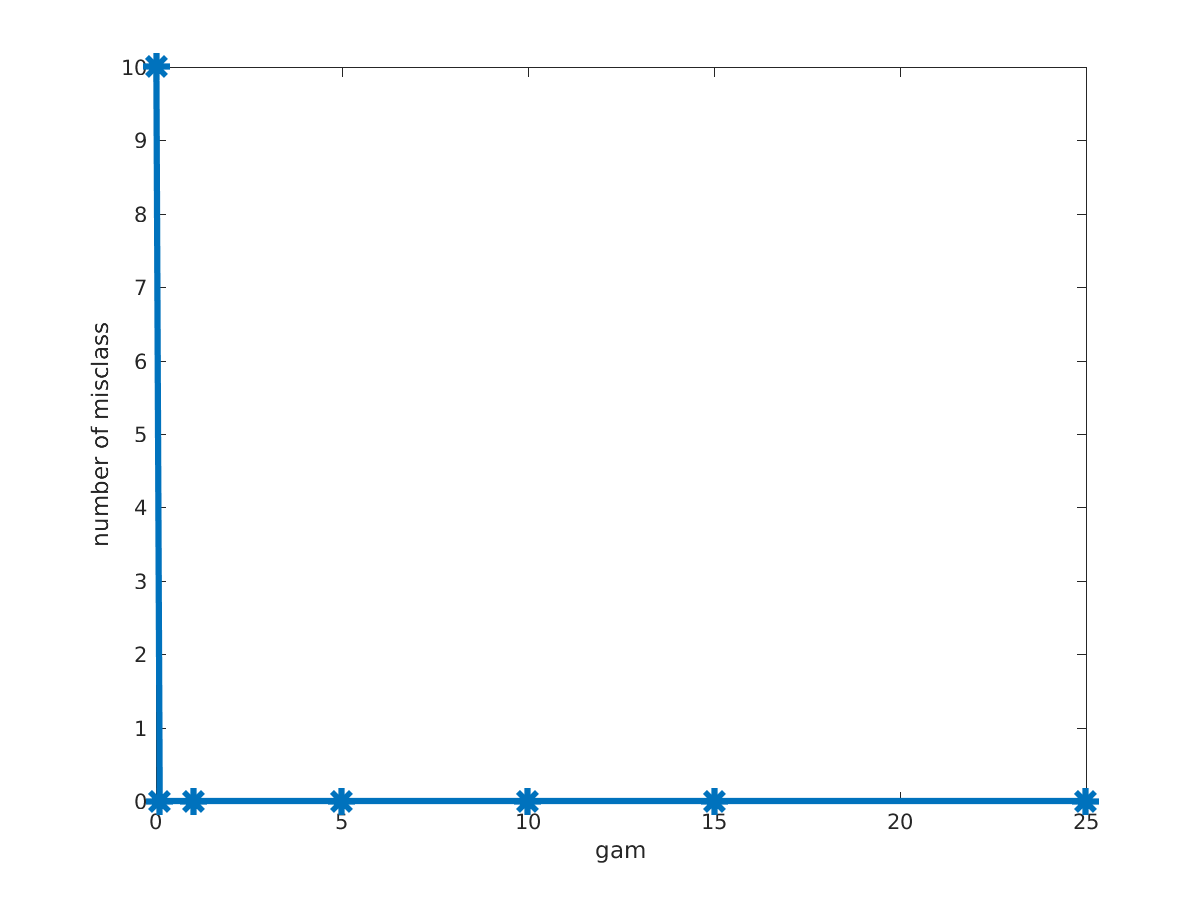
\includegraphics[width = \textwidth]{iris-rbf-gam-rate.png}
		\caption{$n_{misclass}$ vs $\gamma$}
	\end{subfigure}
\caption{Iris classification: RBF kernel with $\sigma^2 = 1$ (fixed) and different values for the hyperparameter $\gamma$ set to 1 (a), 25 (b) and the plot of $n_{misclass}$ as a function of $\gamma$ on the test set.}
\label{iris-rbf-gam}
\end{figure}

For the $\gamma$ parameters and this dataset assuming $\sigma^2 = 1$, a good range seems to be between 0.1 and 10 since beyond that point the region for class 2 kept getting smaller. At smaller $\gamma$ values, the region is quite large. However in practice this will be different for different datasets. In the next subsection, automated tuning algorithms for hyperparameter optimization are explored. 

\subsubsection{Choice of hyperparameters}

We continue with the Iris dataset in this section. First, the training set from the previous section ($n=100$) is further divided into a training set ($n=80$) and a validation set ($n=20$). The model is trained on the training and set and then evaluated on the validation set. The results are shown below in figure \ref{iris-rbf-fixed-val}. We cannot use this validation set, however, to measure the final model since the error rate obtained will be biased (underestimated) since the model has already "seen" the data, so to speak. In the figures, we see that the error rate shows a large amount of variation for different $(\gamma, \sigma^2)$ values and determining an optimal combination that will generalize well to future data remains a mystery.\\

\begin{figure}[ht]
\centering
	\begin{subfigure}[b]{0.3\textwidth}
		\centering
		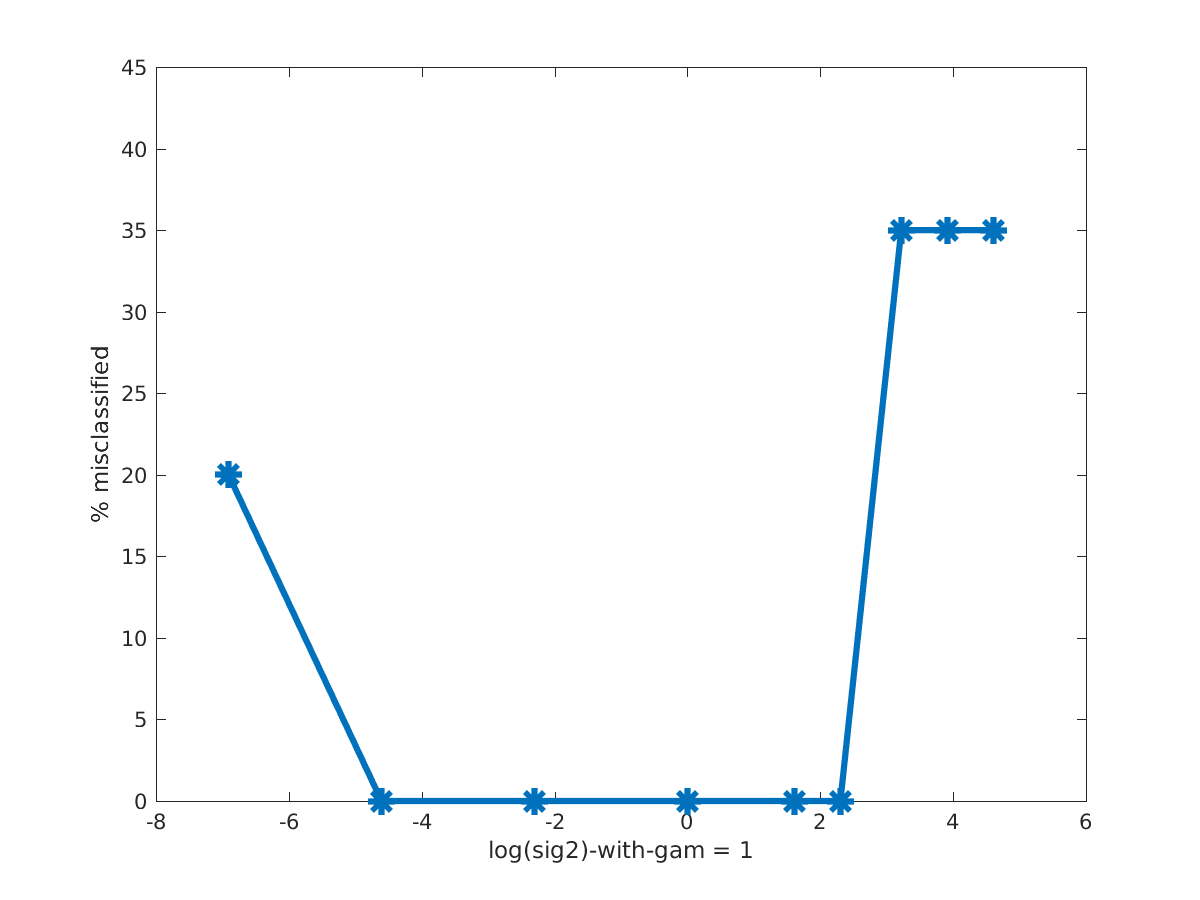
\includegraphics[width = \textwidth]{iris-rbf-fixed-val-gam-1.png}
		\caption{$\gamma = 1$}
	\end{subfigure}%
	\begin{subfigure}[b]{0.3\textwidth}
		\centering
		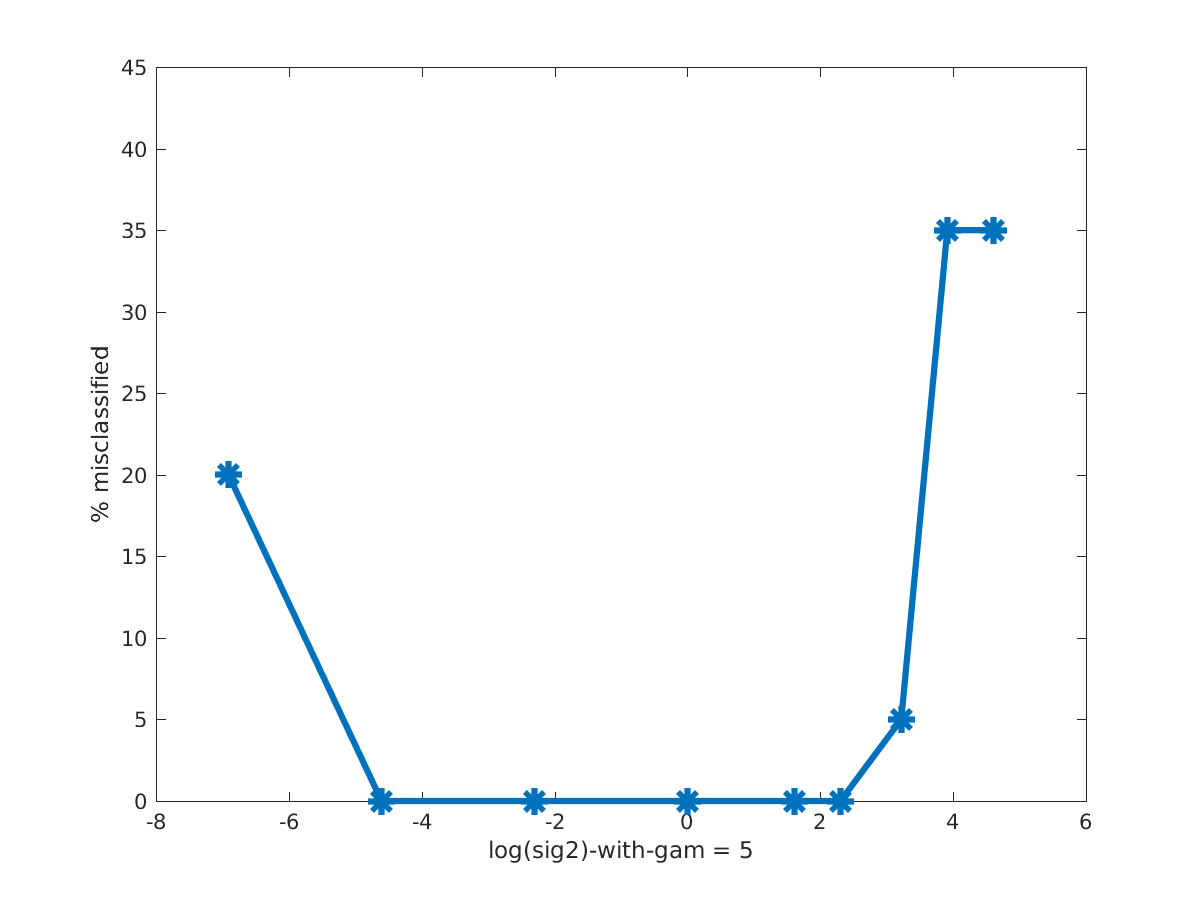
\includegraphics[width = \textwidth]{iris-rbf-fixed-val-gam-5.png}
		\caption{$\gamma = 5$}
	\end{subfigure}%
	\begin{subfigure}[b]{0.3\textwidth}
		\centering
		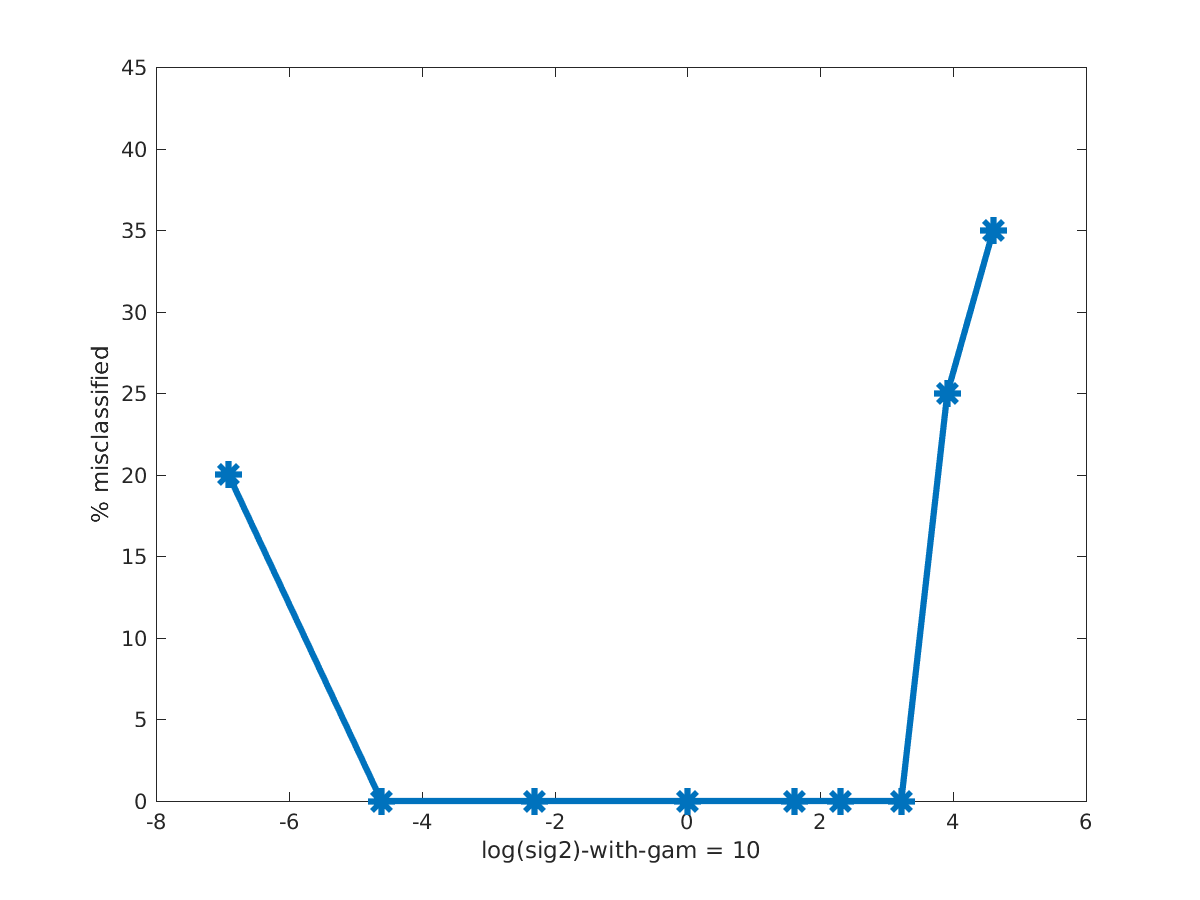
\includegraphics[width = \textwidth]{iris-rbf-fixed-val-gam-10.png}
		\caption{$\gamma = 10$}
	\end{subfigure}
		\begin{subfigure}[b]{0.3\textwidth}
		\centering
		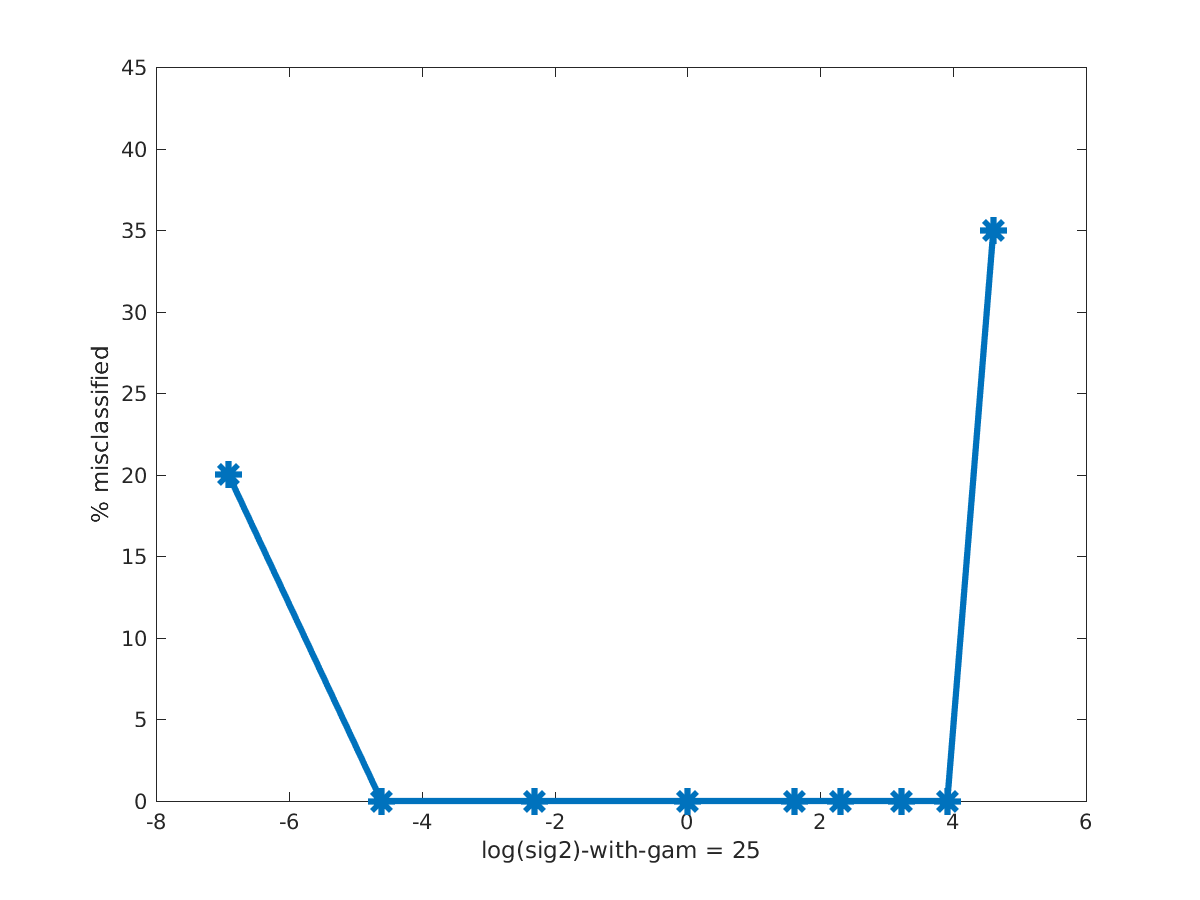
\includegraphics[width = \textwidth]{iris-rbf-fixed-val-gam-25.png}
		\caption{$\gamma = 25$}
	\end{subfigure}%
	\begin{subfigure}[b]{0.3\textwidth}
		\centering
		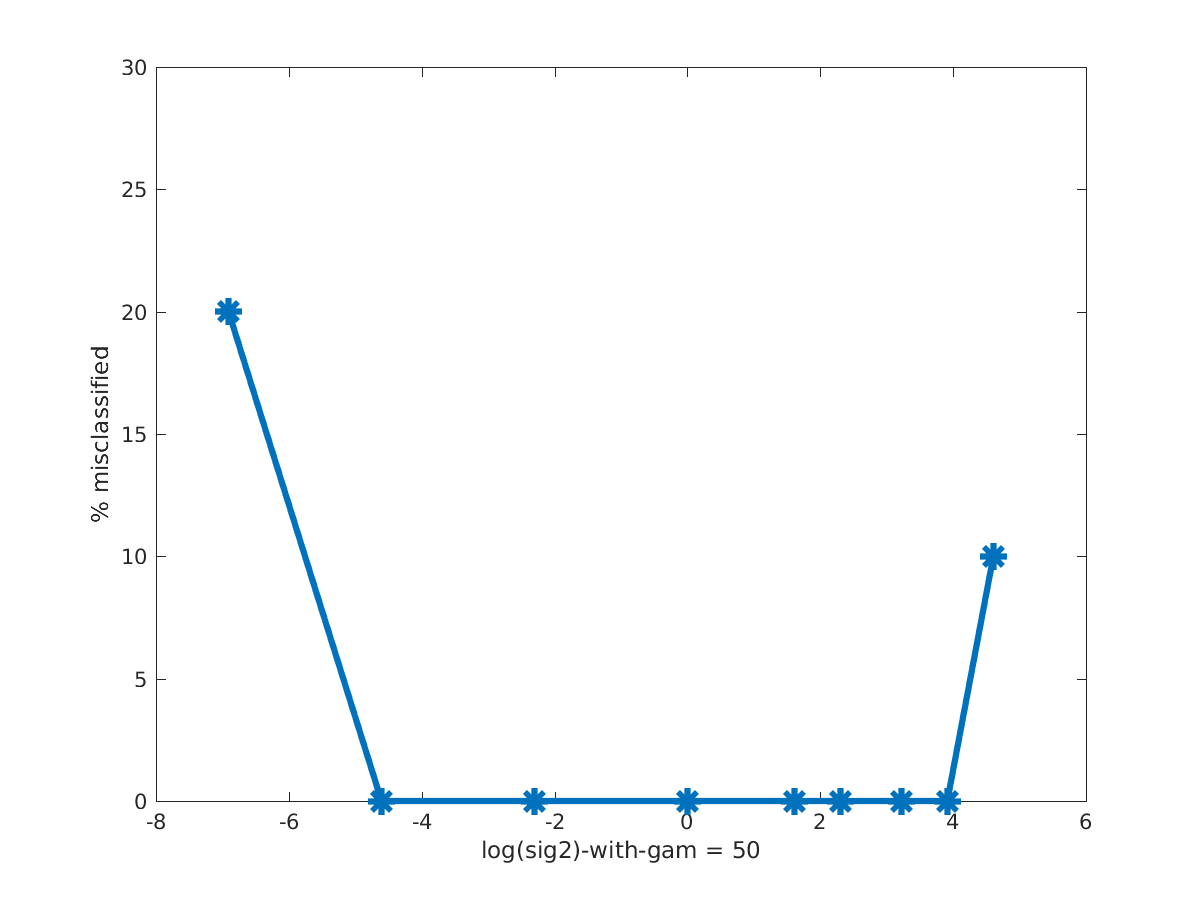
\includegraphics[width = \textwidth]{iris-rbf-fixed-val-gam-50.png}
		\caption{$\gamma = 50$}
	\end{subfigure}%
	\begin{subfigure}[b]{0.3\textwidth}
		\centering
		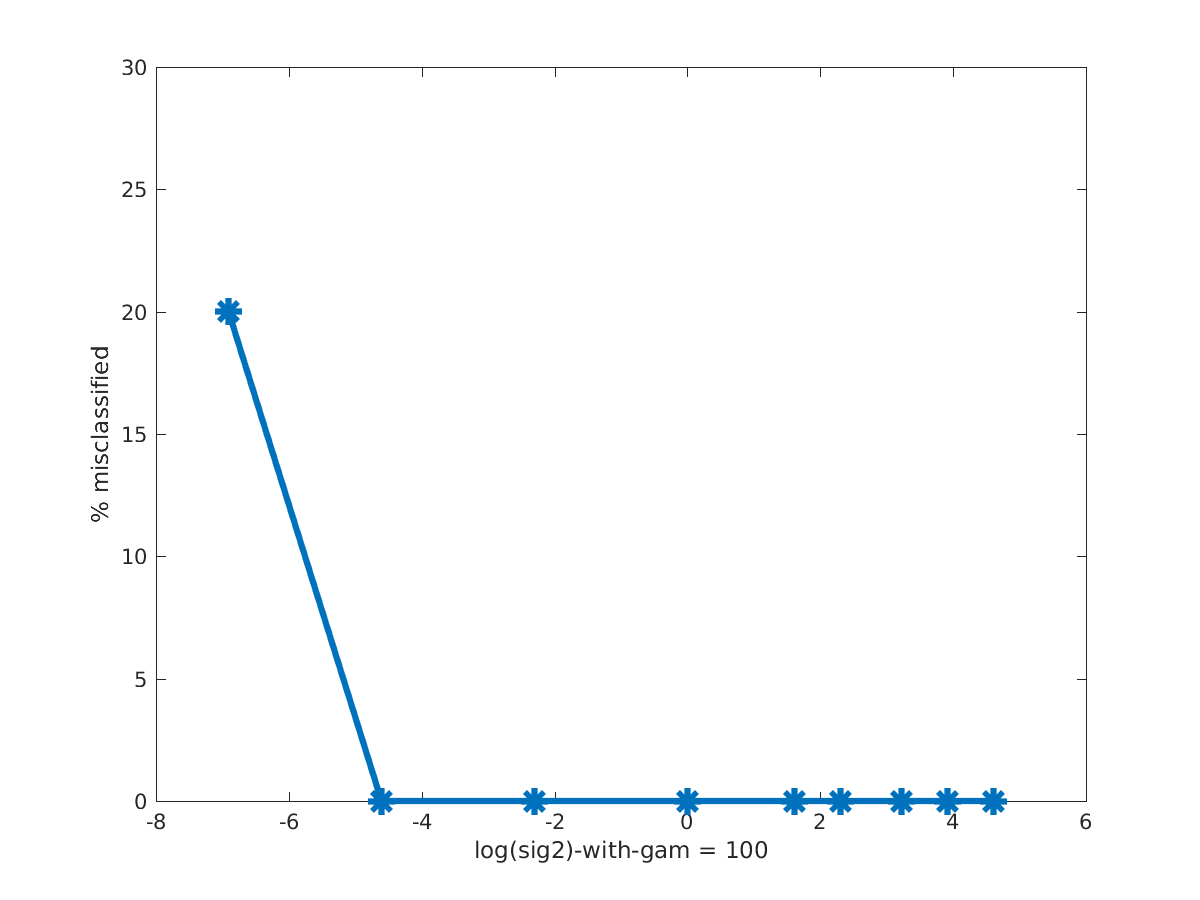
\includegraphics[width = \textwidth]{iris-rbf-fixed-val-gam-100.png}
		\caption{$\gamma = 100$}
	\end{subfigure}
\caption{Iris classification (fixed validation set): RBF kernel with different log($\sigma^2$) values at each level of $\gamma \in \{1,5,10,25,50,100\}$ values. The error rates (\% observations in the validation set that are misclassified) are plotted for the different $(\gamma, \sigma^2)$ values.)}
\label{iris-rbf-fixed-val}
\end{figure}

One problem with this approach, i.e, splitting the training data into a training and a validation set is that although the split was random, the validation set may (by chance) display characteristics either similar or dissimilar to the training set. An alternative approach is performing $k$-fold CV (say $k=10$) where the training set is split into $k$ (disjoint) subsets and at each step of training, $k-1$-subsets are used to build the model and the model is then evaluated on the $k^{th}$ subset that was kept aside as the validation set. We can then select the value of $(\gamma, \sigma^2)$ that lead to the smallest average error rate over the $k$-folds. These figures are plotted in figure \ref{iris-rbf-cv}.\\

\begin{figure}[ht]
\centering
	\begin{subfigure}[b]{0.3\textwidth}
		\centering
		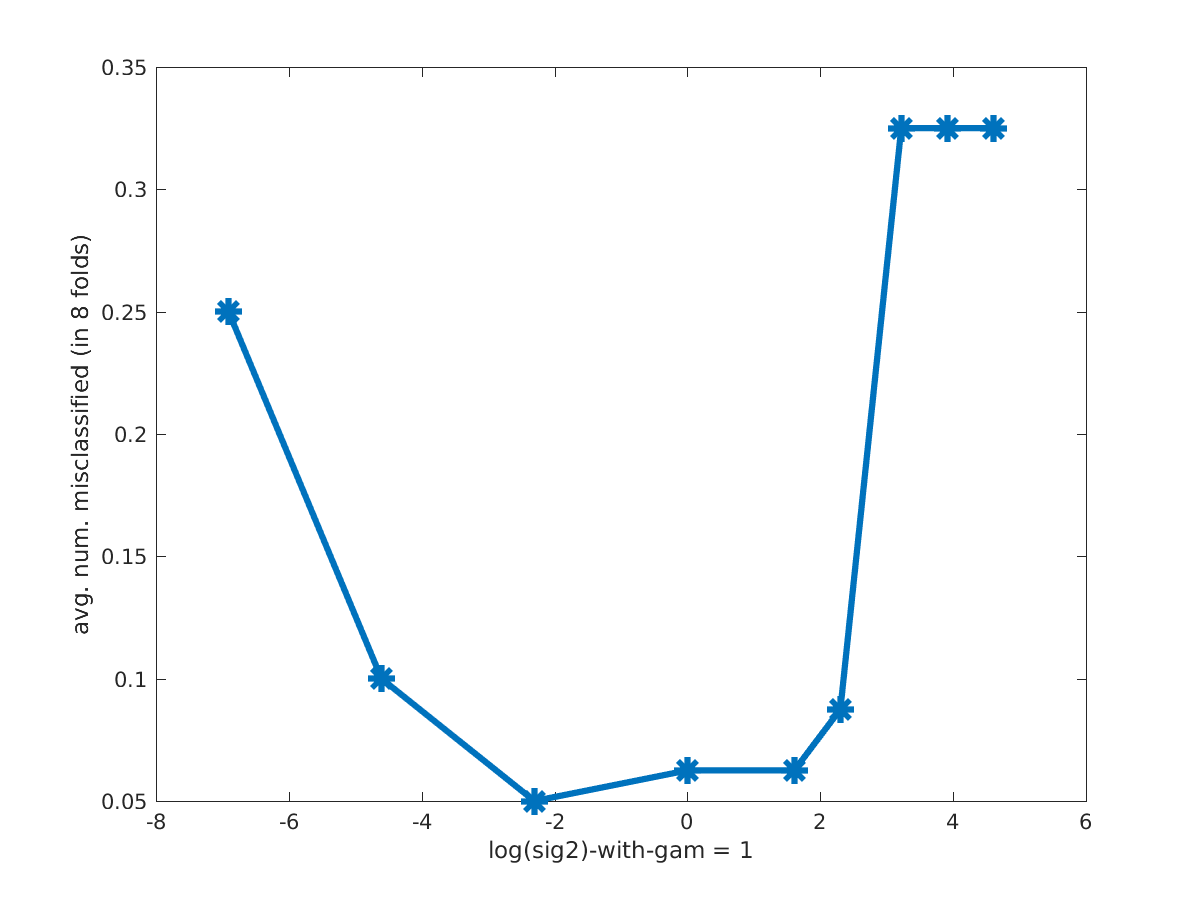
\includegraphics[width = \textwidth]{iris-rbf-cv-gam-1.png}
		\caption{$\gamma = 1$}
	\end{subfigure}%
	\begin{subfigure}[b]{0.3\textwidth}
		\centering
		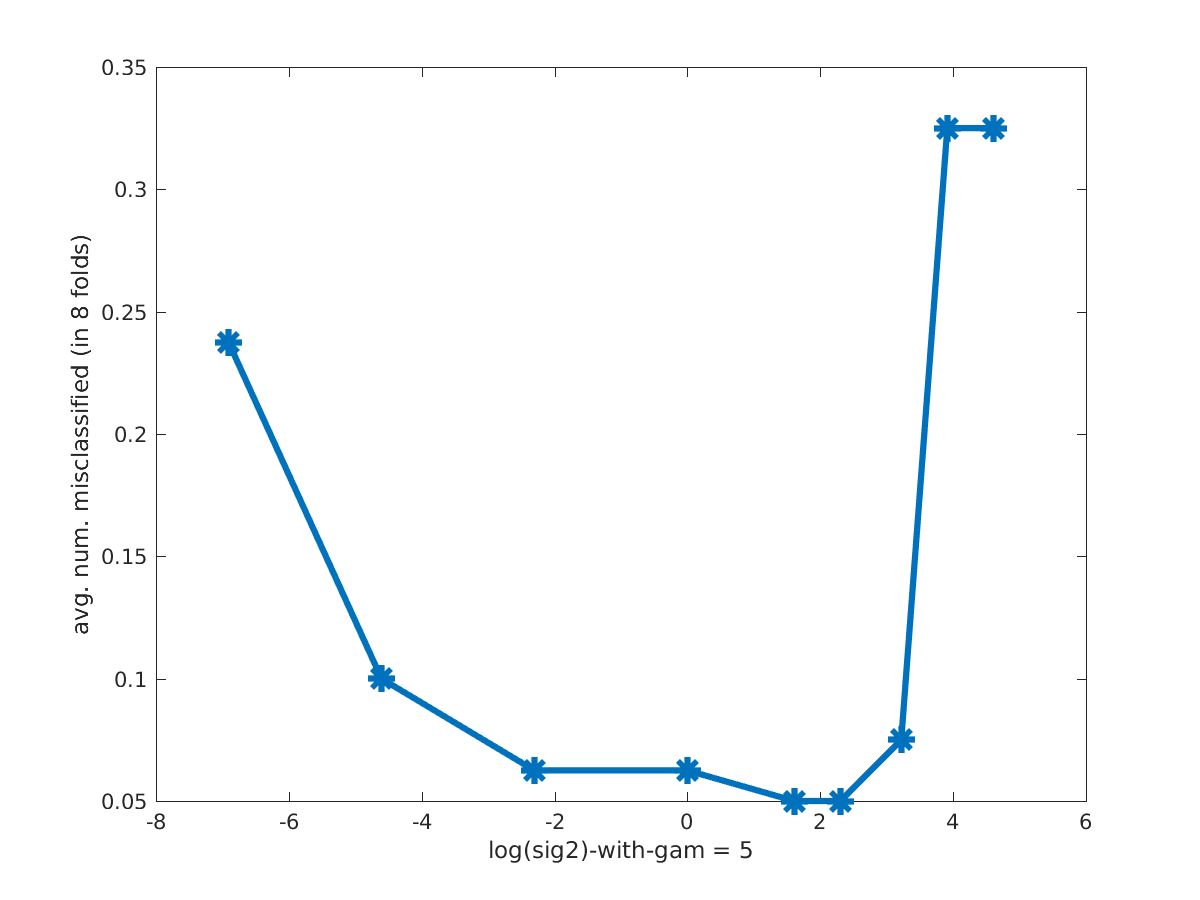
\includegraphics[width = \textwidth]{iris-rbf-cv-gam-5.png}
		\caption{$\gamma = 5$}
	\end{subfigure}%
	\begin{subfigure}[b]{0.3\textwidth}
		\centering
		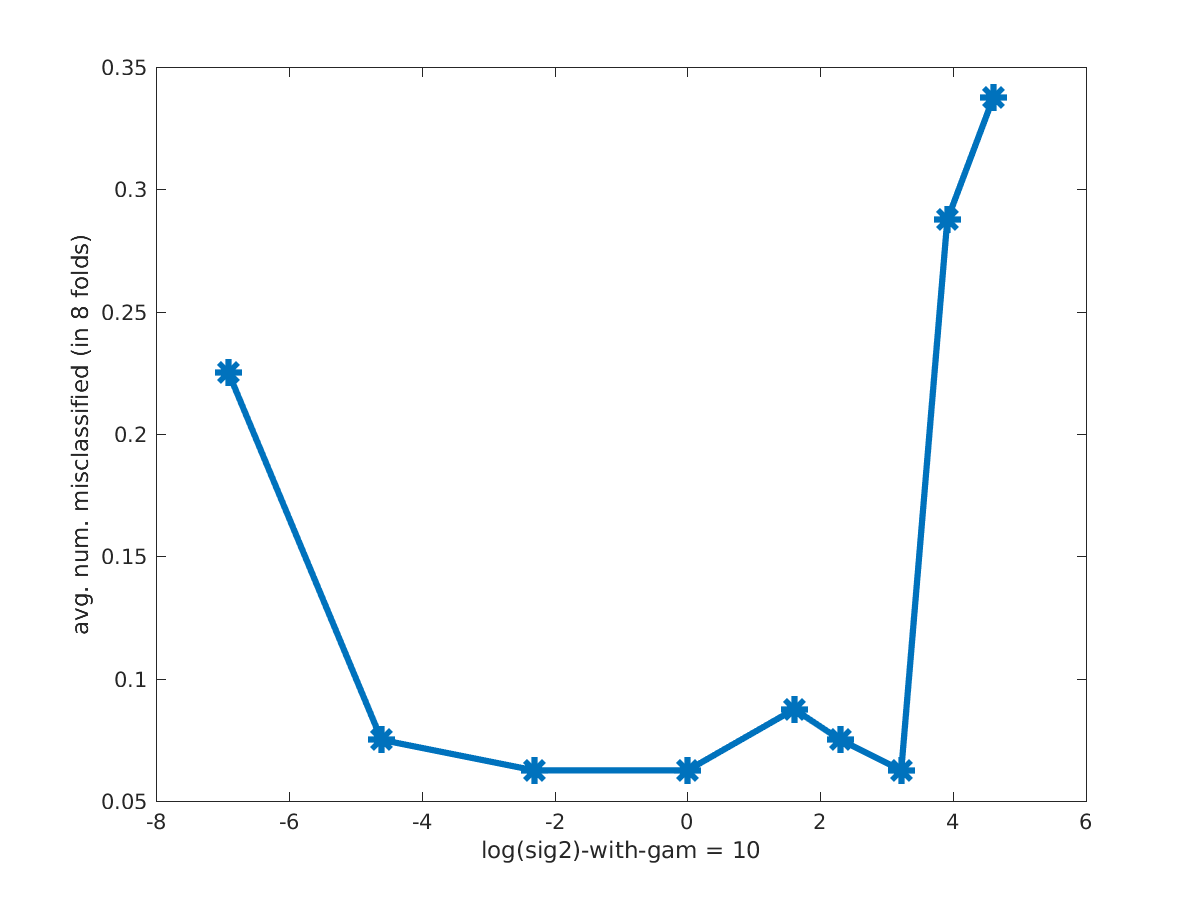
\includegraphics[width = \textwidth]{iris-rbf-cv-gam-10.png}
		\caption{$\gamma = 10$}
	\end{subfigure}
		\begin{subfigure}[b]{0.3\textwidth}
		\centering
		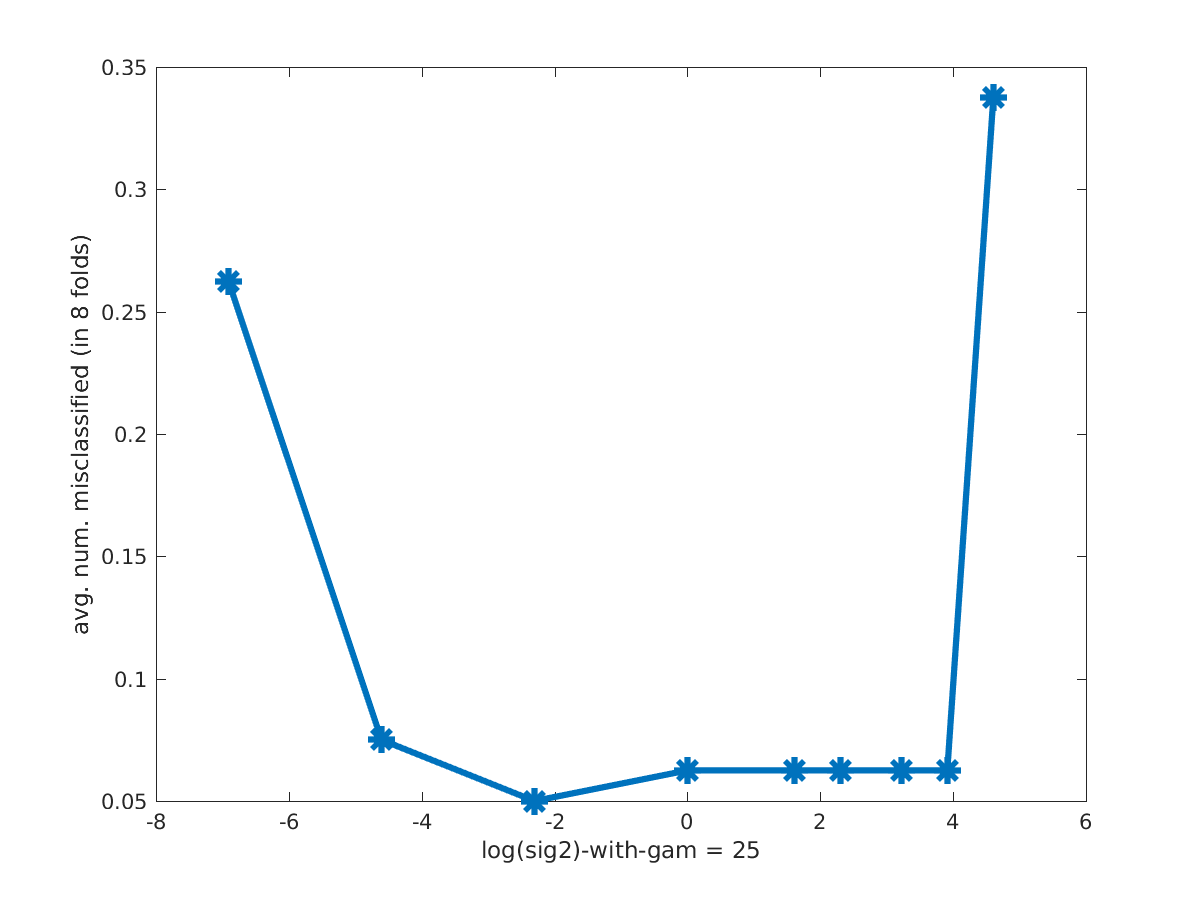
\includegraphics[width = \textwidth]{iris-rbf-cv-gam-25.png}
		\caption{$\gamma = 25$}
	\end{subfigure}%
	\begin{subfigure}[b]{0.3\textwidth}
		\centering
		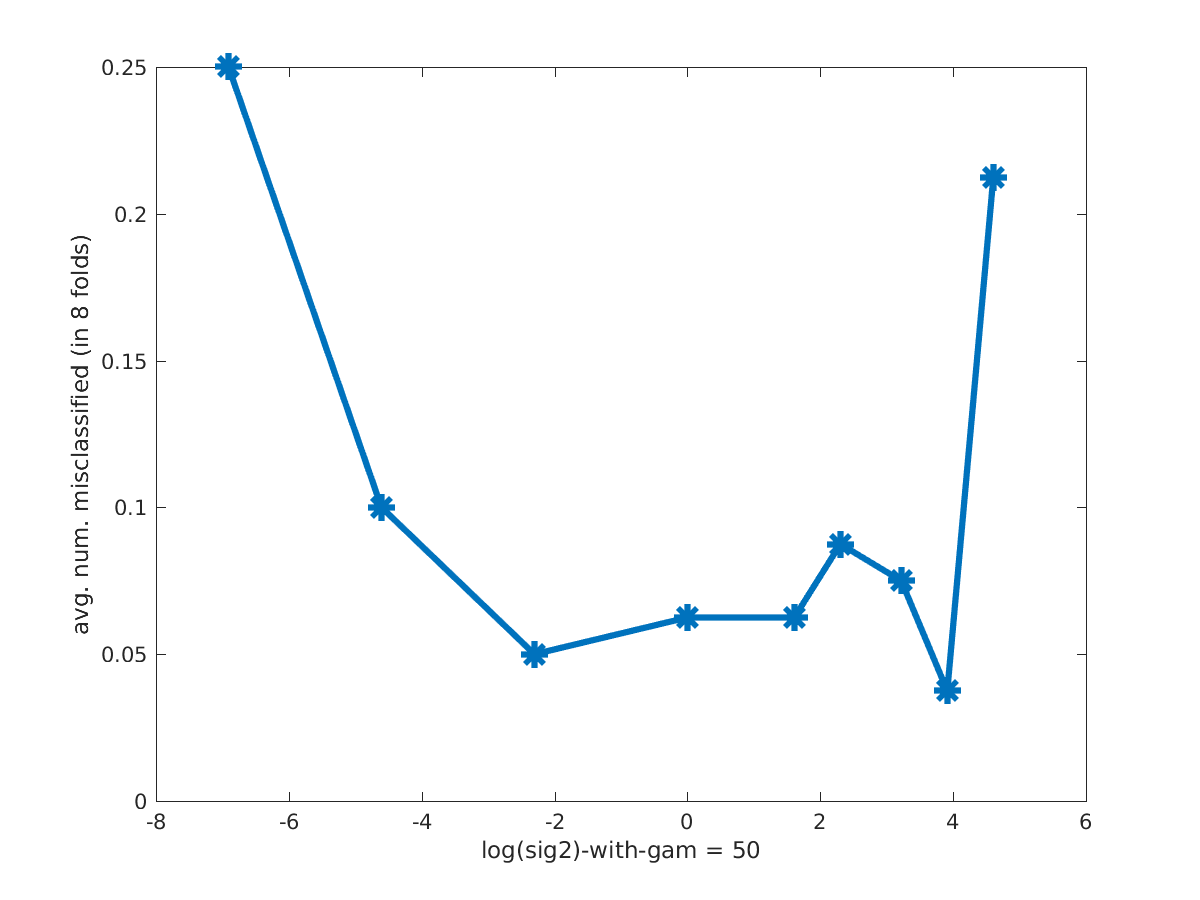
\includegraphics[width = \textwidth]{iris-rbf-cv-gam-50.png}
		\caption{$\gamma = 50$}
	\end{subfigure}%
	\begin{subfigure}[b]{0.3\textwidth}
		\centering
		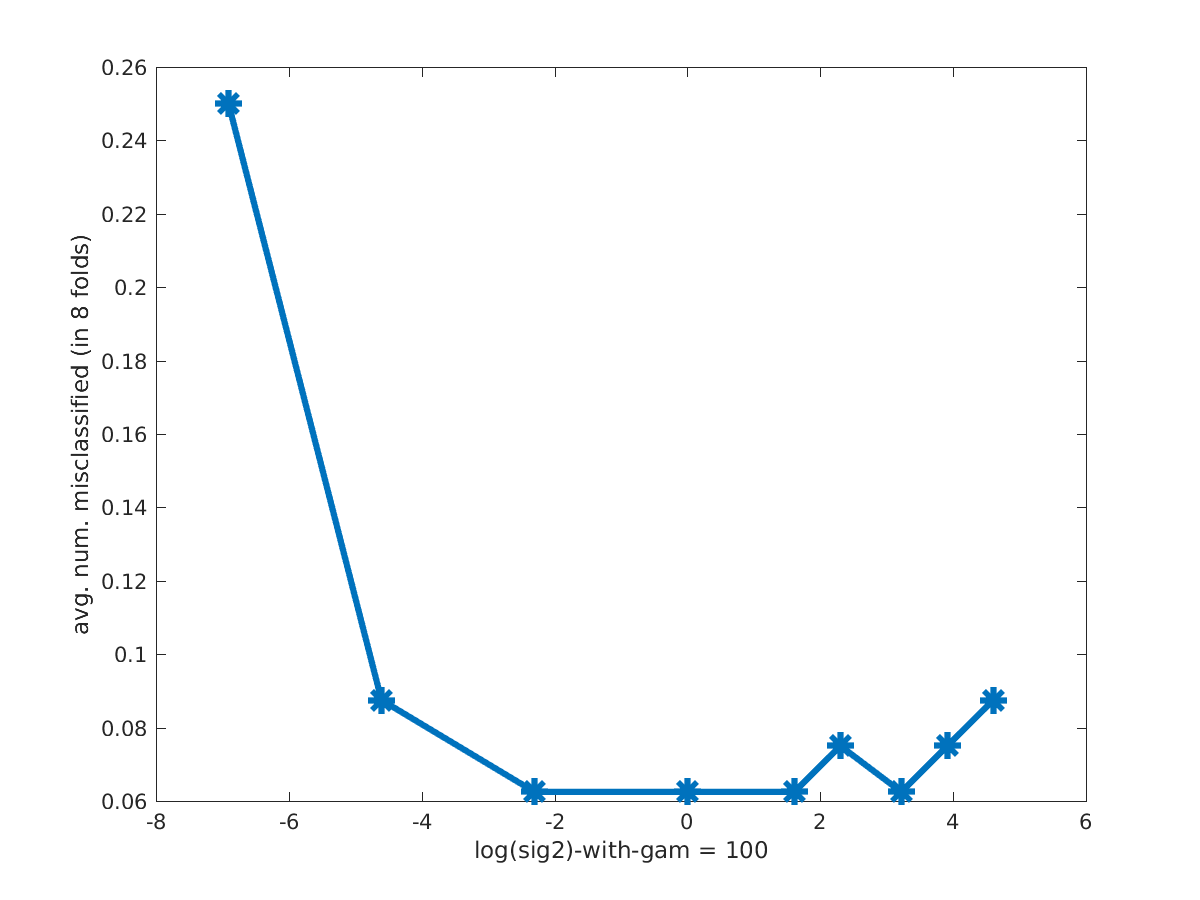
\includegraphics[width = \textwidth]{iris-rbf-cv-gam-100.png}
		\caption{$\gamma = 100$}
	\end{subfigure}
\caption{Iris classification (10-fold crossvalidation): RBF kernel with different log($\sigma^2$) values at each level of $\gamma \in \{1,5,10,25,50,100\}$ values. The average number (across all the folds) of misclassified observations are plotted for the different $(\gamma, \sigma^2)$ values.)}
\label{iris-rbf-cv}
\end{figure}

The $y$-axis does not display the error rate (\% misclassified) but the mean (across the folds) of the number of misclassified observations with each fold used as the validation set. It can be seen that in all the cases, a good value of $\sigma^2$ is 0.01 and all the $\gamma$ values tried seems to result in a good fit (although if a single value had to be selected, $\gamma = 100$ seems to be a good choice). Next, we repeat the procedure but instead of $k$-fold CV, we perform leave-one-out CV (LOOCV) and the results are plotted in figure \ref{iris-rbf-loocv}. It is observed that the misclassification rate is nearly the same as the $k$-fold CV procedure, however, for larger datasets, $k$-fold cv is less computationally intensive as compared to LOOCV and is to be preferred. For smaller datasets (such as this one), it is more sensible to use LOOCV since splitting up the data into folds results in each fold having too few observations.\\

Next, the usage of \texttt{tunelssvm} function is explored to determine optimal tuning parameters. We see that the girdsearch + ds (randomized directional search) method gives the lowest misclassification rate, however, all the algorithms seem to give varying result. The misclassification rate varied a little across multiple runs of each algorithm but the $(\gamma, \sigma^2)$ displayed large variation. This may be a consequence of multiple local minima and each random start of the algorithm results in a local minima. 

\begin{figure}[ht]
\centering
	\begin{subfigure}[b]{0.3\textwidth}
		\centering
		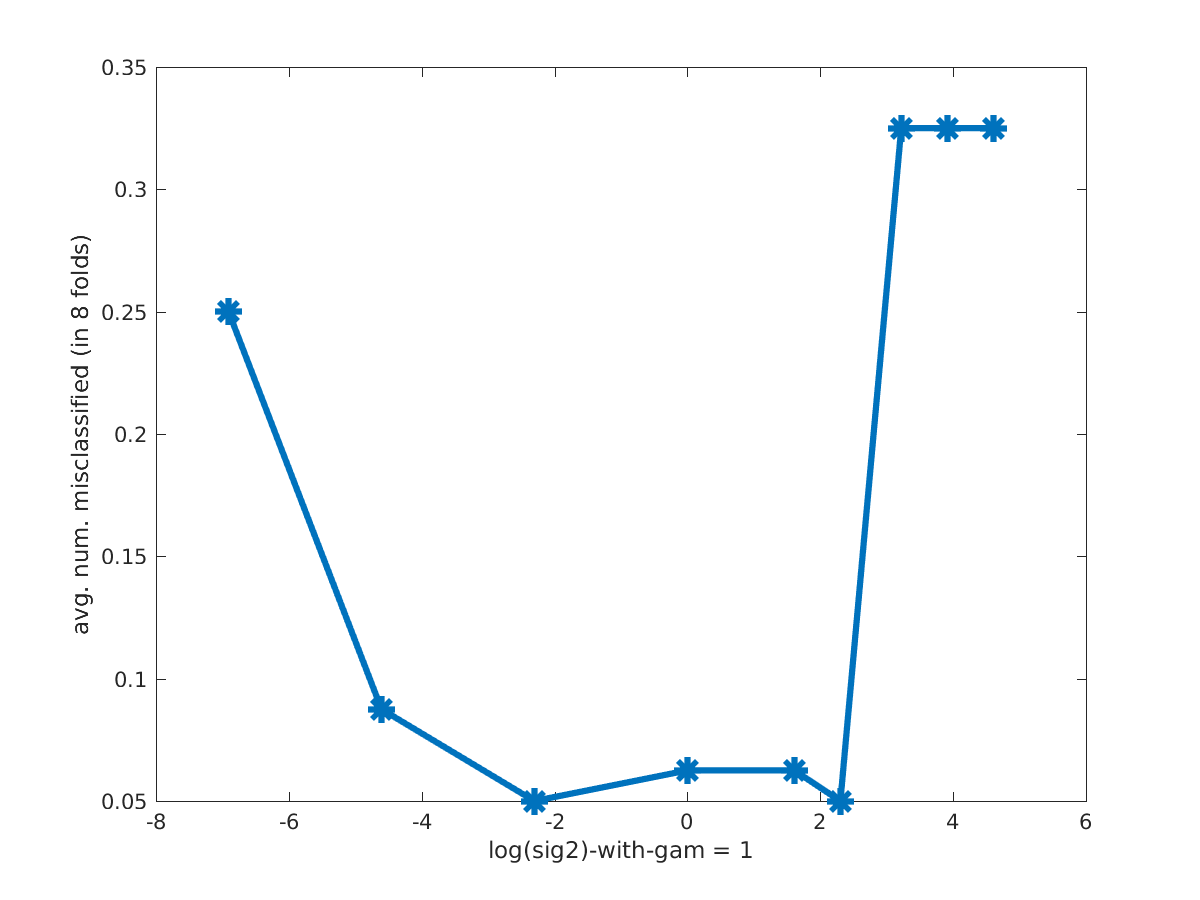
\includegraphics[width = \textwidth]{iris-rbf-loocv-gam-1.png}
		\caption{$\gamma = 1$}
	\end{subfigure}%
	\begin{subfigure}[b]{0.3\textwidth}
		\centering
		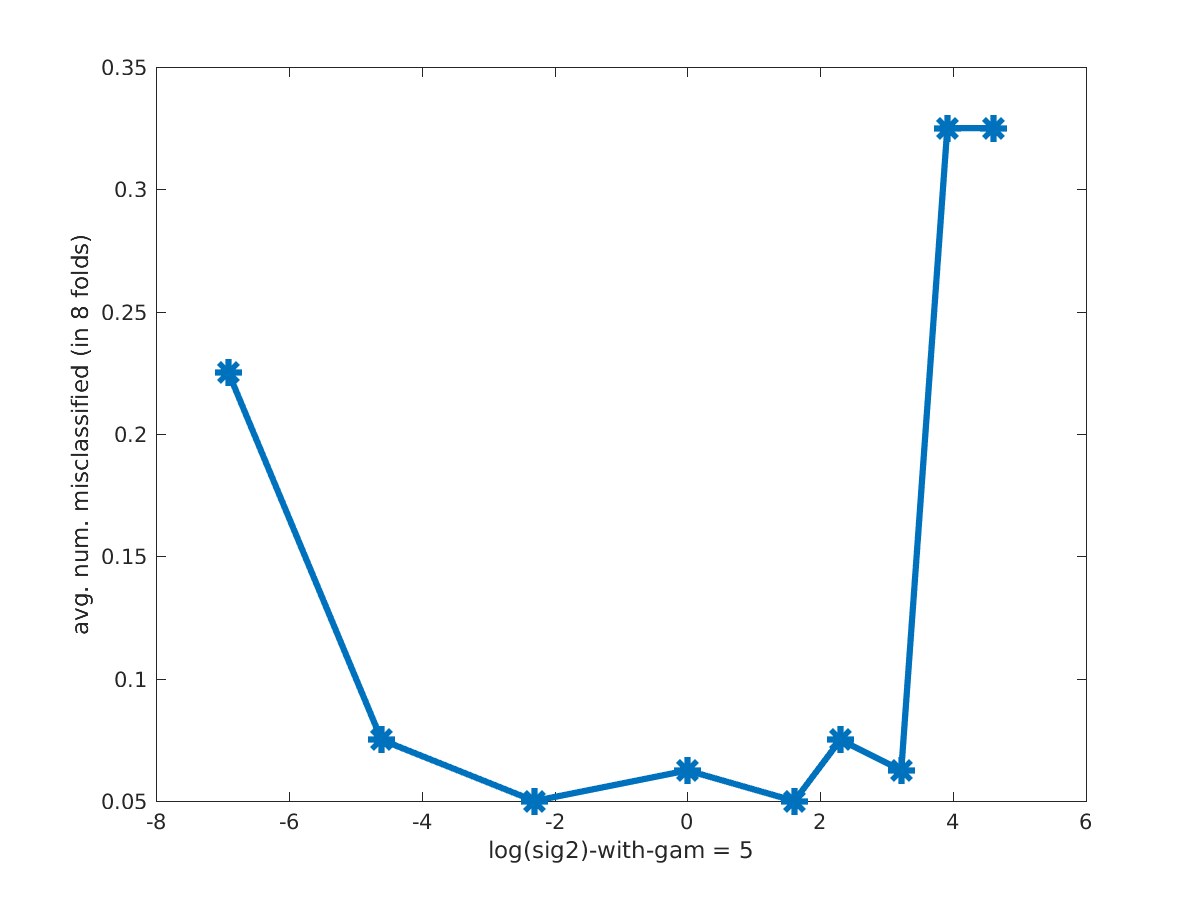
\includegraphics[width = \textwidth]{iris-rbf-loocv-gam-5.png}
		\caption{$\gamma = 5$}
	\end{subfigure}%
	\begin{subfigure}[b]{0.3\textwidth}
		\centering
		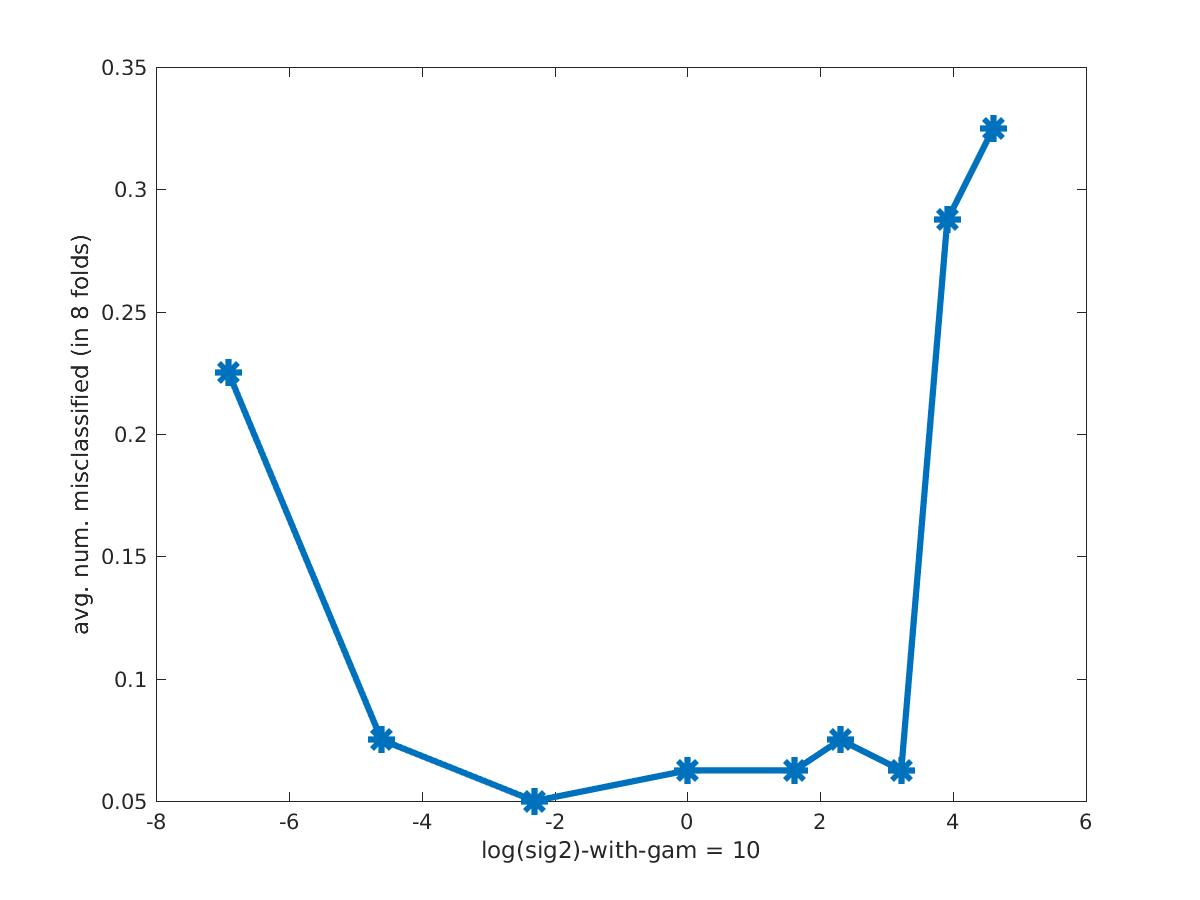
\includegraphics[width = \textwidth]{iris-rbf-loocv-gam-10.png}
		\caption{$\gamma = 10$}
	\end{subfigure}
		\begin{subfigure}[b]{0.3\textwidth}
		\centering
		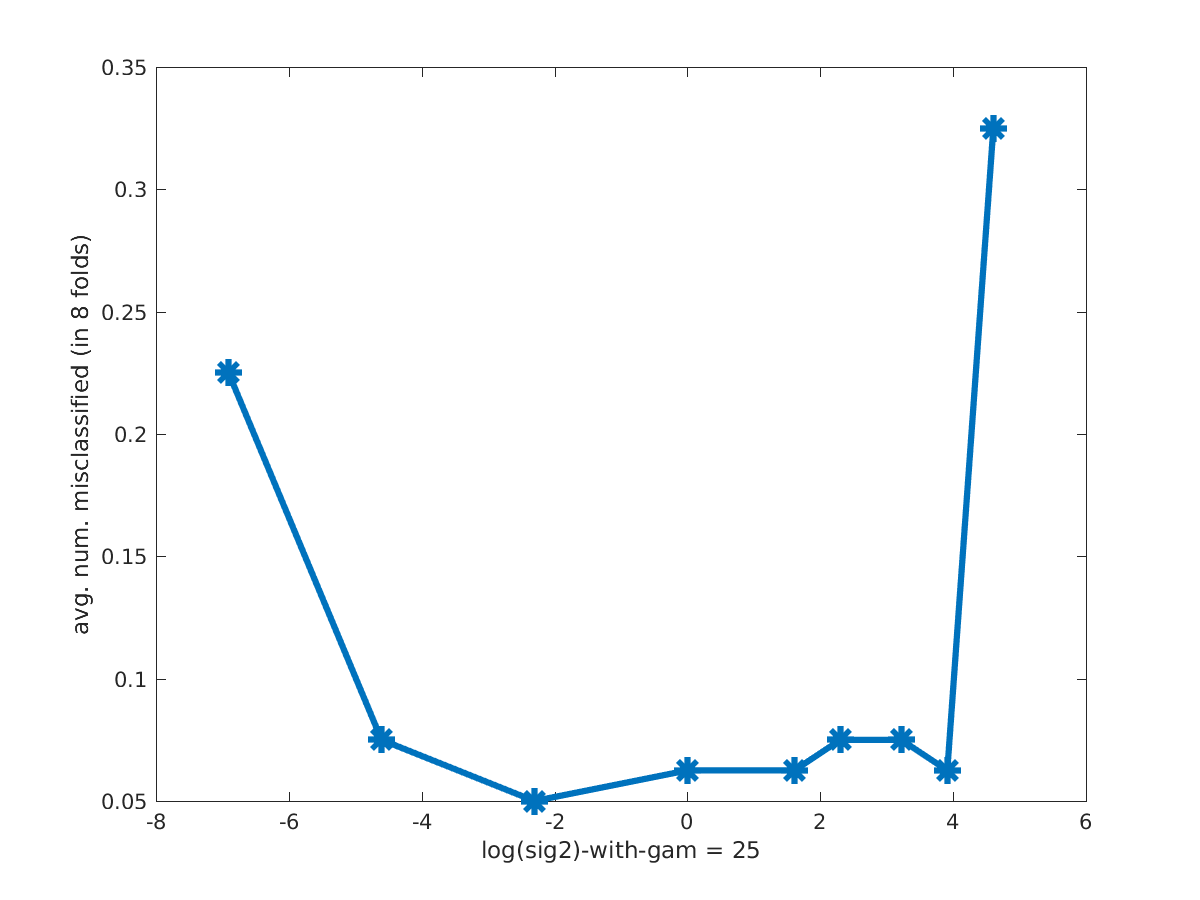
\includegraphics[width = \textwidth]{iris-rbf-loocv-gam-25.png}
		\caption{$\gamma = 25$}
	\end{subfigure}%
	\begin{subfigure}[b]{0.3\textwidth}
		\centering
		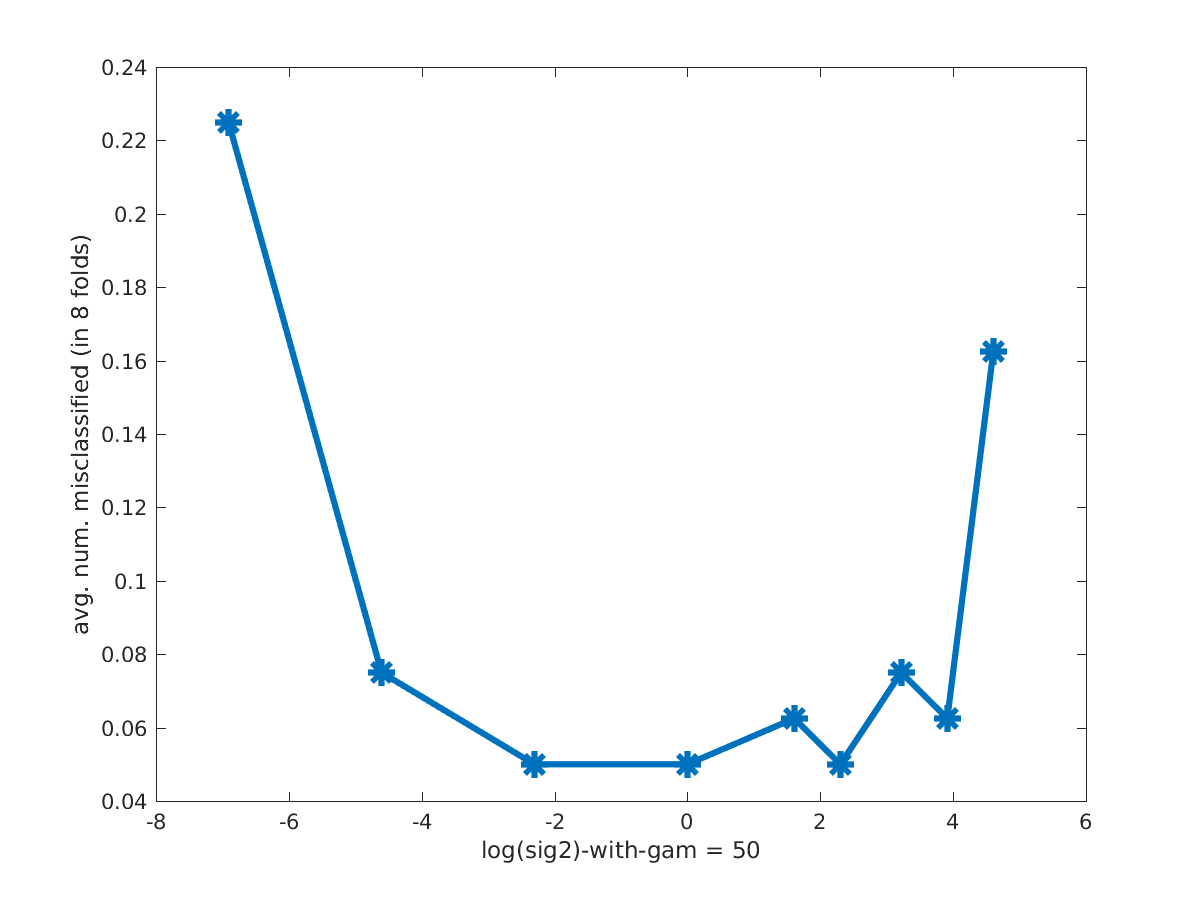
\includegraphics[width = \textwidth]{iris-rbf-loocv-gam-50.png}
		\caption{$\gamma = 50$}
	\end{subfigure}%
	\begin{subfigure}[b]{0.3\textwidth}
		\centering
		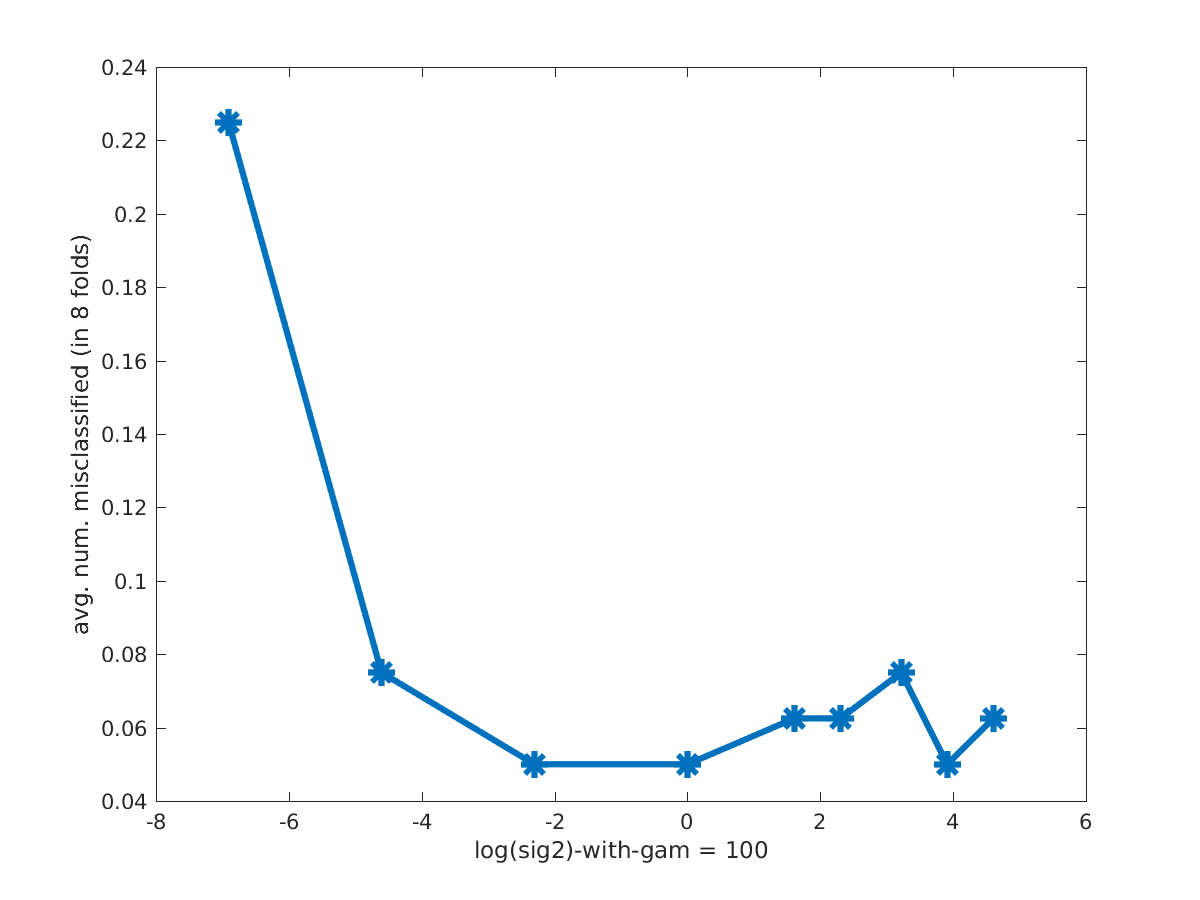
\includegraphics[width = \textwidth]{iris-rbf-loocv-gam-100.png}
		\caption{$\gamma = 100$}
	\end{subfigure}
\caption{Iris classification (leave-one-out crossvalidation (LOOCV)): RBF kernel with different log($\sigma^2$) values at each level of $\gamma \in \{1,5,10,25,50,100\}$ values. The average number (across all the folds) of misclassified observations are plotted for the different $(\gamma, \sigma^2)$ values.)}
\label{iris-rbf-loocv}
\end{figure}

\begin{table}[ht]
\centering
\begin{tabular}{|c|c|c|c|}
\hline
Method & Misclassification rate & $\gamma$ & $\sigma^2$ \\
\hline
simplex + csa & 0.04 & 167.82 & 1.05 \\
simplex + ds & 0.05 & 8.92 & 2.38 \\
gridsearch + csa & 0.04 & 7.55 & 0.05 \\
gridsearch + ds & 0.02 & 0.51 & 8.38 \\
\hline
\end{tabular}
\caption{Misclassification results and optimal hyperparameter values as chosen by the \texttt{tunelssvm} function using different methods.}
\label{iris-tune}
\end{table}

We can also visually assess the performance of a classifier using ROC (receiver operating characteristic) curve. This curve is usually plotted for the classification accuracy of a classifier on the validation set because using the training set will give a biased estimate of the classification accuracy since the classifier has used the training data to build the model. This is why a separate validation set needs to be used for the ROC curve (and for assessing the model in general).

\subsection{Homework Problems}

For each of the datasets, we do the following: plot the training and test data, try a linear SVM, try an RBF kernel and tune the parameters and plot the ROC curve. 

\subsubsection{Ripley Dataset}

The training ($n = 250$) and test ($n = 1000$)  sets are plotted in figure \ref{ripley-data}. This dataset is easy to visualize since it only has 2 features. From the training and test sets we see that the datasets are to a large extent quite easily separable with few overlapping points. Both the linear and RBF kernel can be expected to perform quite well here. The classification accuracy (as seen in the ROC curves in figure \ref{ripley-roc}) for the linear kernel is 95.9\% and 96.9\% for the RBF kernel. Both have similar performance but RBF leads to a higher accuracy, albeit by a small margin. Furthermore, similar to the previous cases, the performance of the classifiers remains the same despite the combination of hyperparameter values varying by a large amount at each iteration of \texttt{tunelssvm}.

\begin{figure}[ht]
\centering
	\begin{subfigure}[b]{0.5\textwidth}
		\centering
		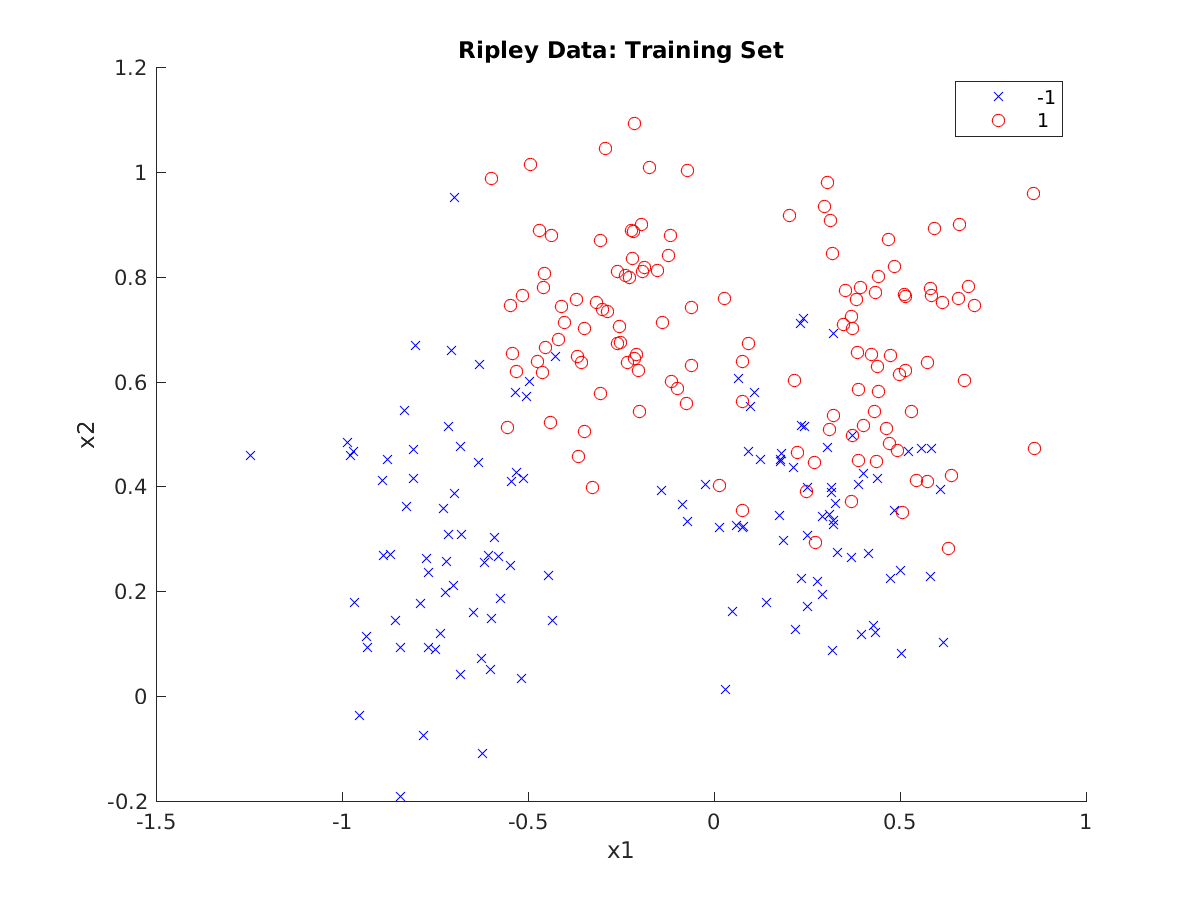
\includegraphics[width = 0.8\textwidth]{ripley-train.png}
		\caption{Training set}
	\end{subfigure}%
	\begin{subfigure}[b]{0.5\textwidth}
		\centering
		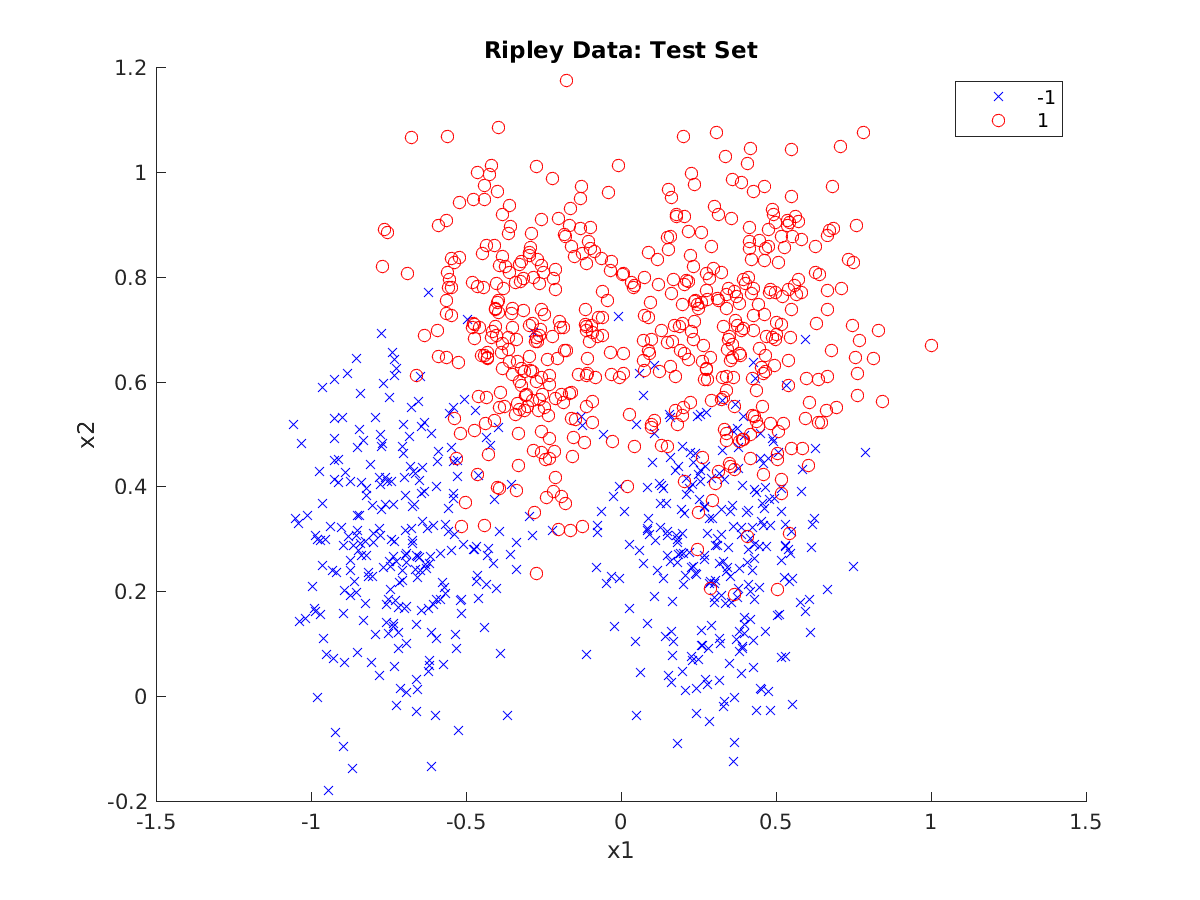
\includegraphics[width = 0.8\textwidth]{ripley-test.png}
		\caption{Test set}
	\end{subfigure}
\caption{Ripley classification: Training and test data.}
\label{ripley-data}
\end{figure}

\begin{figure}[ht]
\centering
	\begin{subfigure}[b]{0.5\textwidth}
		\centering
		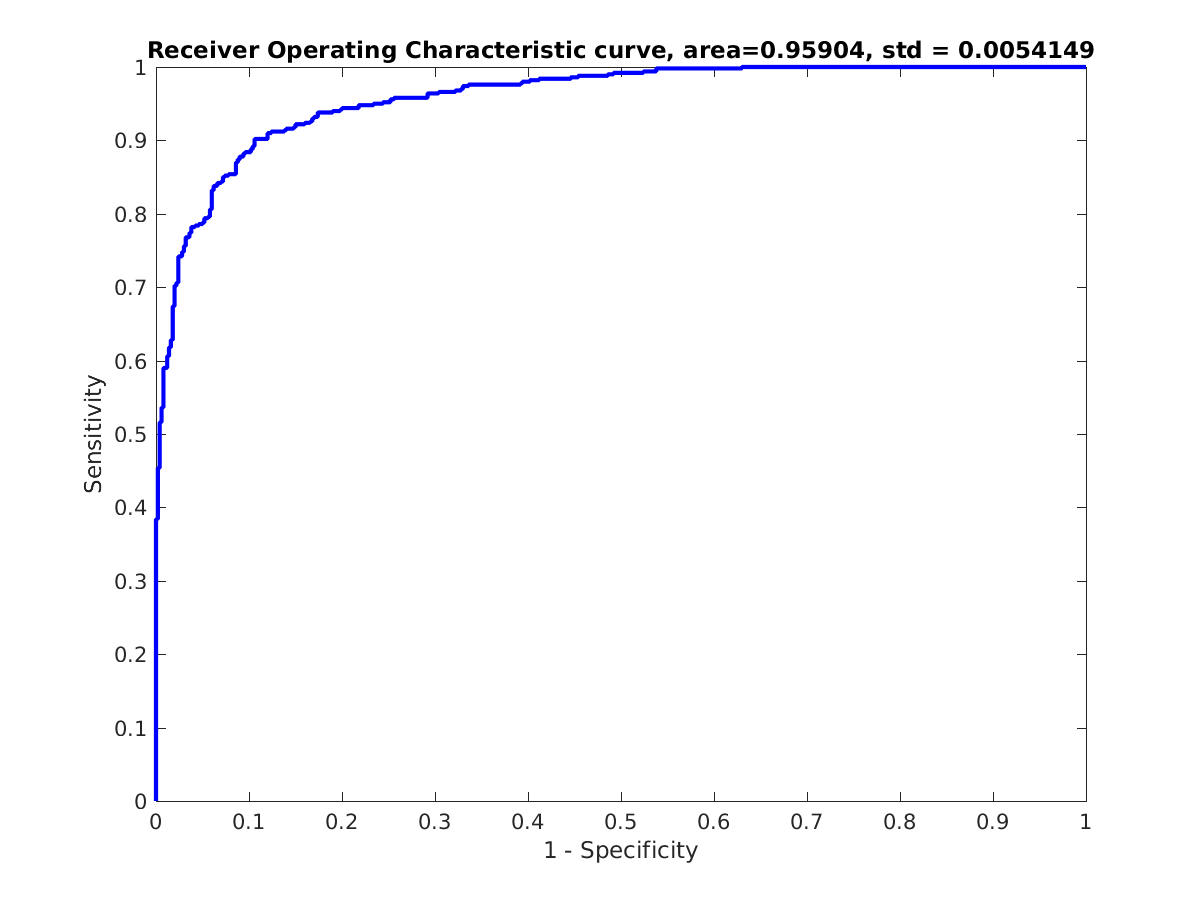
\includegraphics[width = 0.8\textwidth]{ripley-roc-linear.png}
		\caption{Linear Kernel}
	\end{subfigure}%
	\begin{subfigure}[b]{0.5\textwidth}
		\centering
		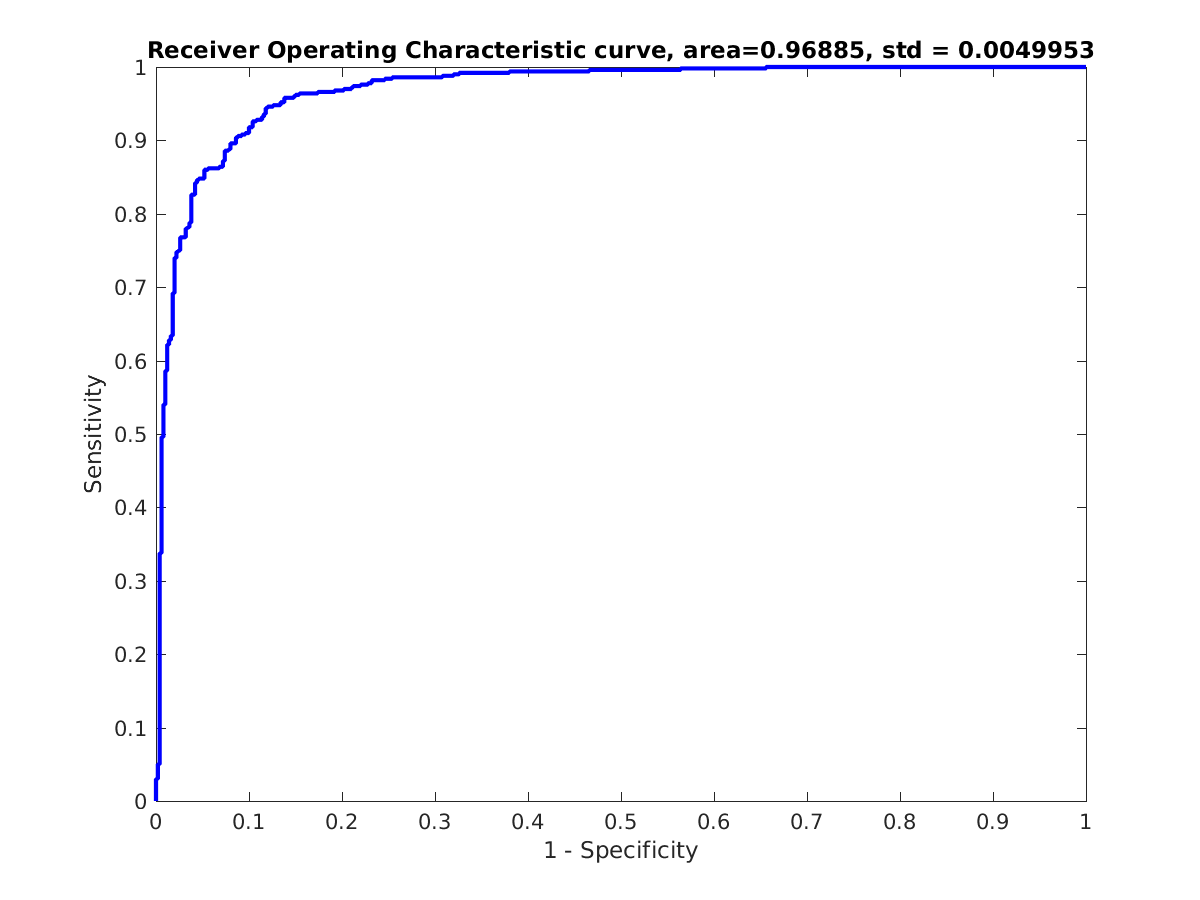
\includegraphics[width = 0.8\textwidth]{ripley-roc-rbf.png}
		\caption{RBF Kernel}
	\end{subfigure}
\caption{Ripley classification: ROC curve for assessing classification accuracy on the test set.}
\label{ripley-roc}
\end{figure}

\subsubsection{Breast Cancer Dataset}

The training ($n = 400$) and test ($n = 169$) sets. This dataset is difficult to visualize since it has 30 features. The classification accuracy (as seen in the ROC curves in figure \ref{boobies-roc}) for the both kernels is 99.56\% which indicates that either kernel can be used but hyperparameter optimization must be performed to obtain the same results. The high accuracy of this method probably indicates that the two classes are quite separated which is why it is easy to assign them the correct class label. Furthermore, similar to the previous cases, the performance of the classifiers remains the same despite the combination of hyperparameter values varying by a large amount at each iteration of \texttt{tunelssvm}.

\begin{comment}
\begin{figure}[ht]
\centering
	\begin{subfigure}[b]{0.5\textwidth}
		\centering
		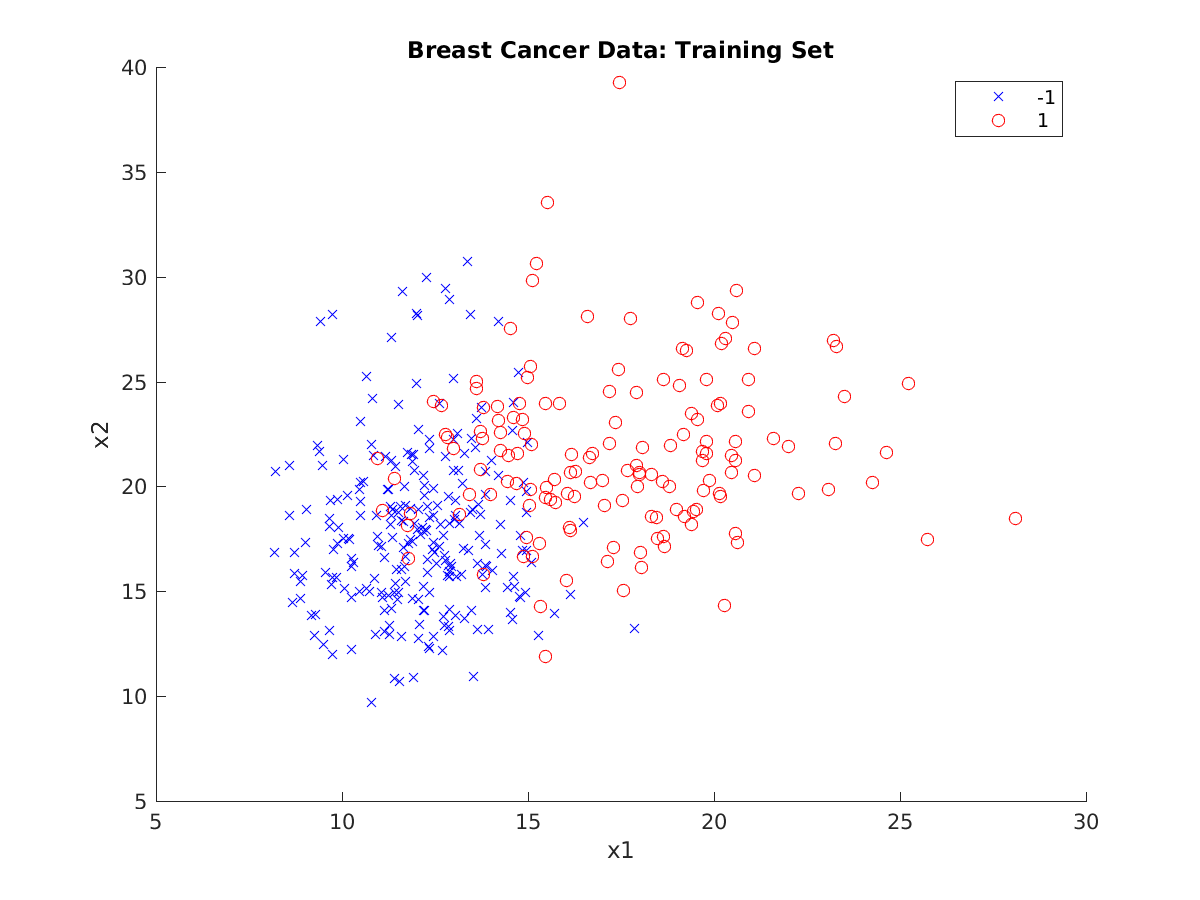
\includegraphics[width = 0.8\textwidth]{breast-train.png}
		\caption{Training set}
	\end{subfigure}%
	\begin{subfigure}[b]{0.5\textwidth}
		\centering
		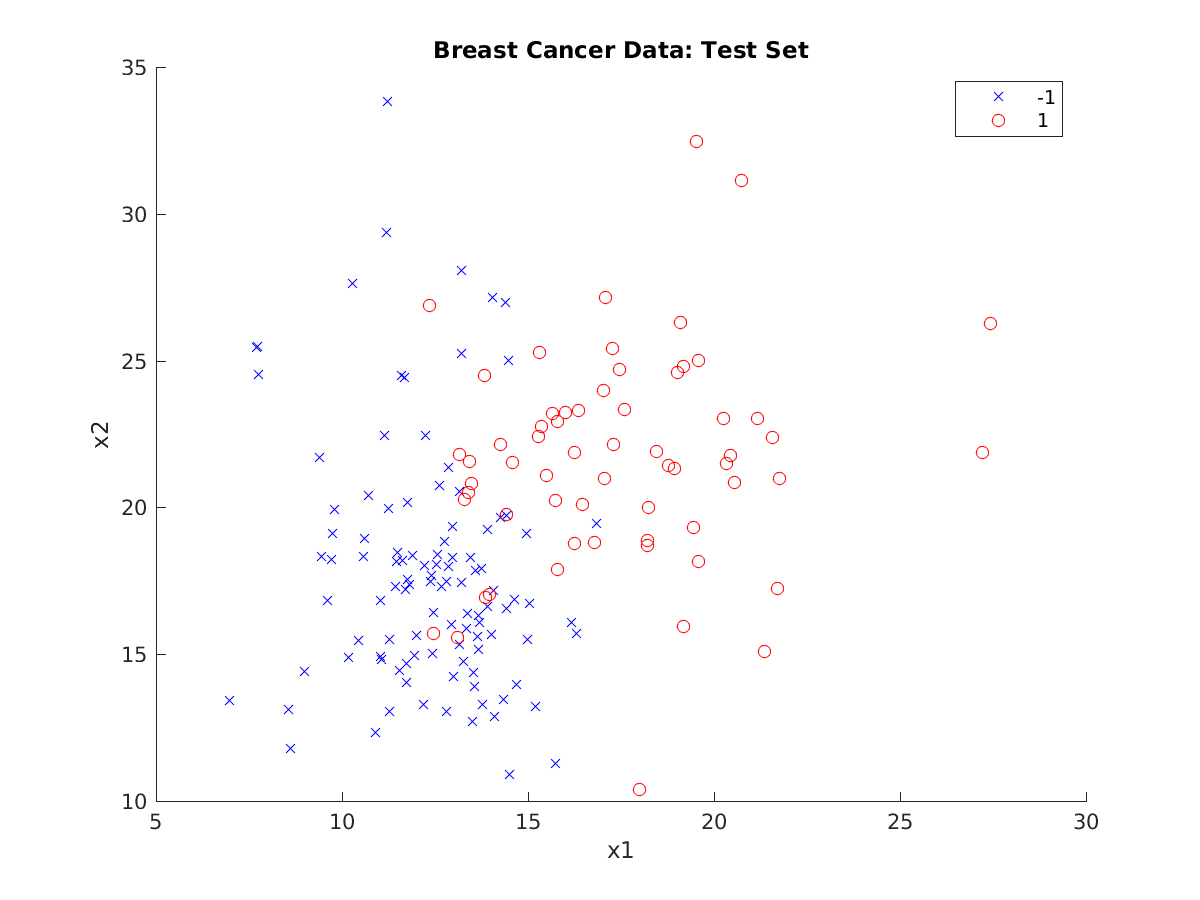
\includegraphics[width = 0.8\textwidth]{breast-test.png}
		\caption{Test set}
	\end{subfigure}
\caption{Breast cancer classification: Training and test data. Only the first two features are plotted since the whole dataset resides in a 30 dimensional (feature) space which cannot be visualized.}
\label{boobies-data}
\end{figure}
\end{comment}

\begin{figure}[ht]
\centering
	\begin{subfigure}[b]{0.5\textwidth}
		\centering
		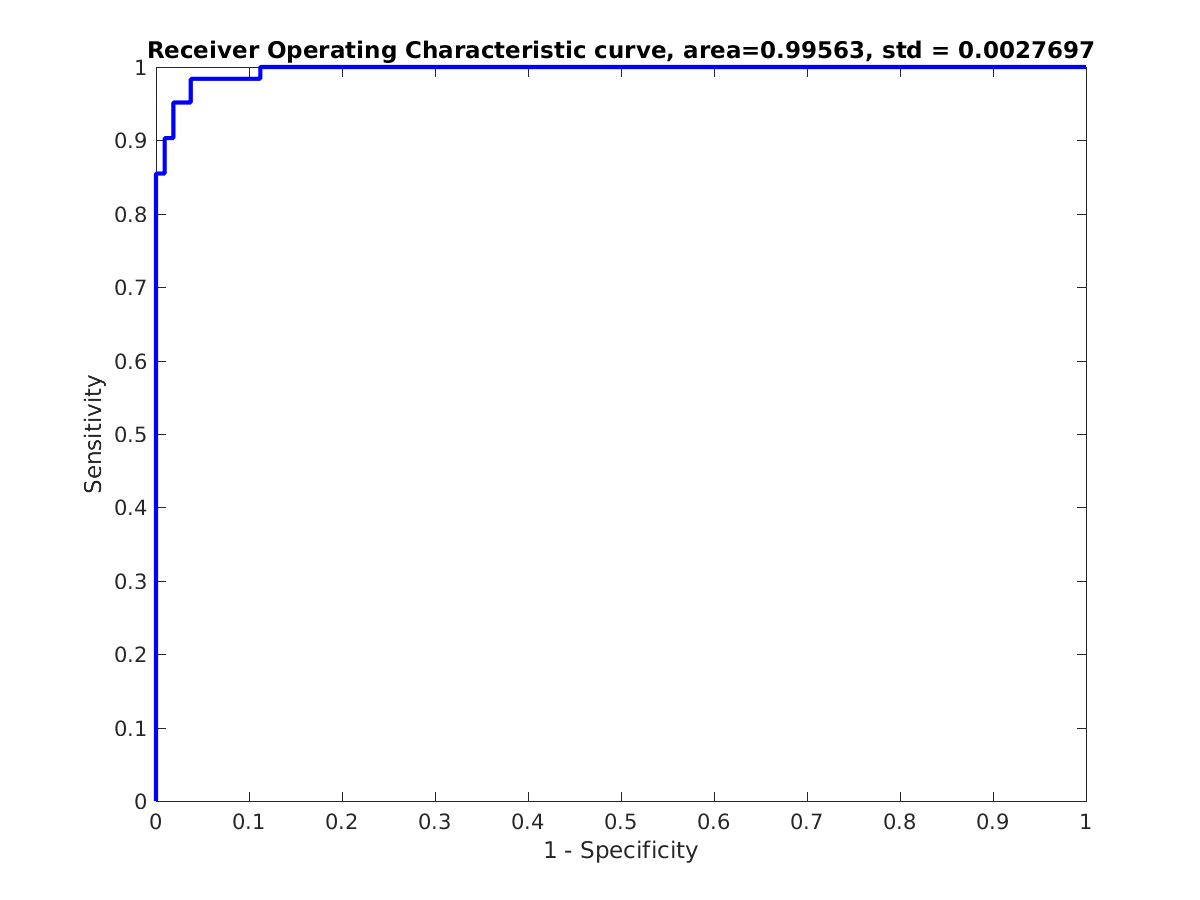
\includegraphics[width = 0.8\textwidth]{breast-roc-linear.png}
		\caption{Linear Kernel}
	\end{subfigure}%
	\begin{subfigure}[b]{0.5\textwidth}
		\centering
		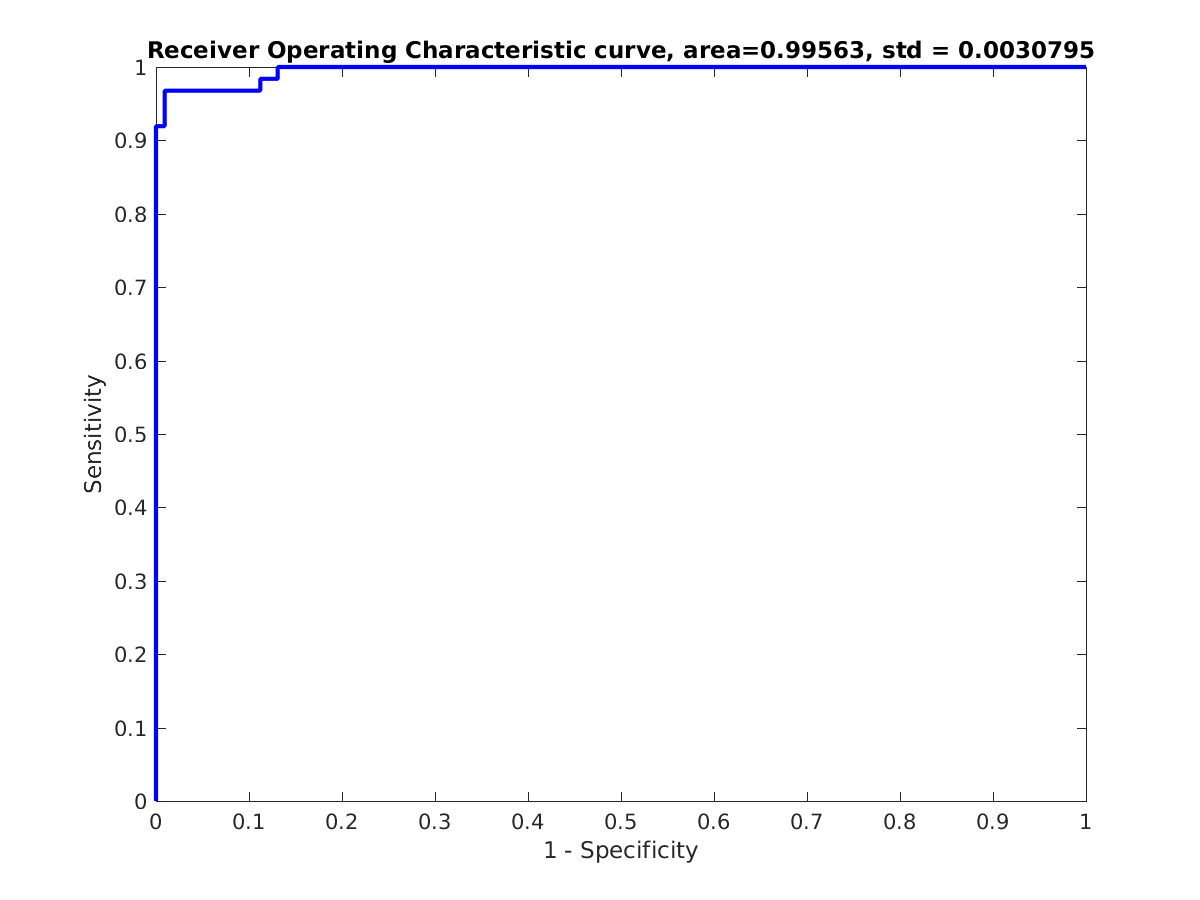
\includegraphics[width = 0.8\textwidth]{breast-roc-rbf.png}
		\caption{RBF Kernel}
	\end{subfigure}
\caption{Breast cancer classification: ROC for the linear and RBF kernels.}
\label{boobies-roc}
\end{figure}

\subsubsection{Diabetes Dataset}

The training ($n = 300$) and test ($n = 168$)  sets. This dataset is difficult to visualize since it has 8 features. We plotted (not shown) the first two features. It was seen from the figures that there was a lot of overlap between the two classes (at least in the subspace of first two features) and this may make it challenging for the classifier to find a separating margin with high accuracy. The classification accuracy (as seen in the ROC curves in figure \ref{diabeetus-roc}) for the linear kernel is 84.4\%  and 85.3\% for the RBF kernel which indicates that the RBF kernel is marginally better. Furthermore, similar to the previous cases, the performance of the classifiers remains the same despite the combination of hyperparameter values varying by a large amount at each iteration of \texttt{tunelssvm}.

\begin{comment}
\begin{figure}[ht]
\centering
	\begin{subfigure}[b]{0.5\textwidth}
		\centering
		\includegraphics[width = 0.8\textwidth]{diabetes-train.png}
		\caption{Training set}
	\end{subfigure}%
	\begin{subfigure}[b]{0.5\textwidth}
		\centering
		\includegraphics[width = 0.8\textwidth]{diabetes-test.png}
		\caption{Test set}
	\end{subfigure}
\caption{PIMA Indians Diabetes classification: Training and test data. The dimension of the feature space is 8 which can't be visualized, thus only the first two features and the corresponding class labels are plotted.}
\label{diabeetus-data}
\end{figure}
\end{comment}

\begin{figure}[ht]
\centering
	\begin{subfigure}[b]{0.5\textwidth}
		\centering
		\includegraphics[width = 0.8\textwidth]{diabetes-roc-lin.png}
		\caption{Linear Kernel}
	\end{subfigure}%
	\begin{subfigure}[b]{0.5\textwidth}
		\centering
		\includegraphics[width = 0.8\textwidth]{diabetes-roc-rbf.png}
		\caption{RBF Kernel}
	\end{subfigure}
\caption{PIMA Indians Diabetes classification: ROC curves for the linear and RBF kernels.}
\label{diabeetus-roc}
\end{figure}

\section{Exercise Session 2: Function Estimation}

The main goal in this exercise is that of function estimation where a SVM is trained for regression (continuous response), not classification (finite response).

\subsection{SVM for Regression}

SVM can not only be used for classification but also regression. We explored the demo \texttt{uiregress} with different settings. Some of the results are shown below in figure \ref{uiregress}.\\

Parameter C determines the trade off between the model complexity (flatness) and the degree to which deviations larger than $\varepsilon$ are tolerated in optimization formulation for example, if C is too large (infinity), then the objective is to minimize the empirical risk only, without regard to model complexity part in the optimization formulation. Parameter $\varepsilon$ on the other hand controls the width of the $\varepsilon$-insensitive zone, used to fit the training data. The value of $\varepsilon$ can affect the number of support vectors used to construct the regression function. The bigger the $\varepsilon$, the fewer support vectors are selected. On the other hand, bigger $\varepsilon$-values results in more 'flat' estimates. Hence, both C and $\varepsilon$-values affect model complexity (but in a different way).
 

\begin{figure}[ht]
\centering
	\begin{subfigure}[b]{0.3\textwidth}
		\centering
		\includegraphics[width = 0.8\textwidth]{reg-e-0-b-inf.png}
		\caption{Linear; $\epsilon = 0$}
	\end{subfigure}%
	\begin{subfigure}[b]{0.3\textwidth}
		\centering
		\includegraphics[width = 0.8\textwidth]{reg-e-05-b-inf.png}
		\caption{Linear; $\epsilon = 0.5$}
	\end{subfigure}%
	\begin{subfigure}[b]{0.3\textwidth}
		\centering
		\includegraphics[width = 0.8\textwidth]{reg-e-025-b-1-poly.png}
		\caption{Poly (3) kernel; $\epsilon = 0.25$}
	\end{subfigure}
	\begin{subfigure}[b]{0.3\textwidth}
		\centering
		\includegraphics[width = 0.8\textwidth]{reg-e-05-sig-01-rbf.png}
		\caption{RBF; $\epsilon = 0.5$, $\sigma^2 = 1$}
	\end{subfigure}%
	\begin{subfigure}[b]{0.3\textwidth}
		\centering
		\includegraphics[width = 0.8\textwidth]{reg-e-05-sig-1-rbf-non.png}
		\caption{RBF; $\epsilon = 0.5$, $\sigma^2 = 1$}
	\end{subfigure}%
	\begin{subfigure}[b]{0.3\textwidth}
		\centering
		\includegraphics[width = 0.8\textwidth]{reg-e-05-sig-001-rbf-non.png}
		\caption{RBF; $\epsilon = 0.5$, $\sigma^2 = 0.01$}
	\end{subfigure}
\caption{SVM for Regression: demo \texttt{uiregress}. Figures (a)-(d) have the same points but different kernels/hyperparameter values. Figures (e) and (f) are on a different nonlinear dataset and performance of the RBF kernel with $\epsilon = 0.5$ (fixed) and $\sigma^2$ values for the hyperparameter are explored.}
\label{uiregress}
\end{figure}

\subsection{Sum of Cosines}

The data in this section is generated as follows: $X \in [-10,10]$ is a sequence of 201 points starting at -10 and ending at 10 with an increment of 0.1. The response vector $Y = cos(X) + cos(2X) + \varepsilon$, $\varepsilon \sim N(0, 0.1^2)$ is the added noise. The dataset is divided into (fixed) training and test sets with the odd indices of $(X,Y)$ taken as the training set and the even indices taken as the test set. We try two ($\gamma, \sigma^2$) values, namely (100, 1.0) and (10, 0.1). An LS-SVM model is trained on the training data with an RBF kernel and evaluated on the test set. The true and predicted values from the test set for the two ($\gamma, \sigma^2$) values are plotted in figure \ref{sum-cos-reg}.\\

 The first set of values (100, 1.0) result in a poor performance on the test set, however the second set of parameter values (10, 0.1) result in a much better performance. However, the question remains: which parameter values result in the optimal performance of the SVM? This is explored in a methodical manner in the next section using the \texttt{tunelssvm} function. Also, experience from the previous session indicates that there is most likely not a single pair of hyperparamter values that is optimal.

\begin{figure}[ht]
\centering
	\begin{subfigure}[b]{0.5\textwidth}
		\centering
		\includegraphics[width = \textwidth]{cos-reg-1.png}
		\caption{$\gamma$ = 100, $\sigma^2$ = 1.0}
	\end{subfigure}%
	\begin{subfigure}[b]{0.5\textwidth}
		\centering
		\includegraphics[width = \textwidth]{cos-reg-2.png}
		\caption{$\gamma$ = 10, $\sigma^2$ = 0.1}
	\end{subfigure}
\caption{Sum of Cosines: Function estimation and evaluation on the test set for the ($\gamma, \sigma^2$) values of the RBF kernel. The LS-SVM model is evaluated on the test set and the known (blue points) and predicted values (red line) are plotted.}
\label{sum-cos-reg}
\end{figure}

\subsection{Hyper-parameter Tuning}

We use the same dataset from the previous subsection. For tuning the model, we try 10-fold crossvalidation ($k$-fold CV) and leave-one-out crossvalidation (LOOCV). In the first part, we create a grid of ($\gamma, \sigma^2$) values and assess the models and fit the ($\gamma, \sigma^2$) values that result in the lowest error on the training set from 10-fold CV and LOO-CV. In the latter half of this section, we use the \texttt{tunelssvm} function to automatically determine the best ($\gamma, \sigma^2$) values and compare different methods within \texttt{tunelssvm}.\\

For the grid search, a subset of values on [-4,5] at increments of 0.1 are taken, which are then used as exponents with base 10 to give the corresponding $\gamma$ and $\sigma^2$ values. Mean squared prediction error (across the folds in CV) is calculated for an SVM fit with each of these ($\gamma, \sigma^2$) values. The ($\gamma, \sigma^2$) value that results in the lowest error is extracted and an SVM model is trained with these values using the training set from the previous section and the performance is evaluated on the test set. These plots are given in figure \ref{tune-grid-test}. It can be useful to visualize the MSE of prediction from the CV procedure as a function of ($\gamma, \sigma^2$) values. These are plotted in figure \ref{tune-grid-contour}.\\

\begin{figure}[ht]
\centering
	\begin{subfigure}[b]{0.5\textwidth}
		\centering
		\includegraphics[width = \textwidth]{tune-grid-err-cv.png}
		\caption{10-fold CV}
	\end{subfigure}%
	\begin{subfigure}[b]{0.5\textwidth}
		\centering
		\includegraphics[width = \textwidth]{tune-grid-err-loo.png}
		\caption{LOO-CV}
	\end{subfigure}
\caption{Sum of Cosines: Contour plots of the average prediction error from the CV procedure for different ($\gamma, \sigma^2$) values (which are plotted on log$_{10}$ scale.}
\label{tune-grid-contour}
\end{figure}

The contour plots indicate that there plenty of ($\gamma, \sigma^2$) values that can give (nearly) optimal results. Although we chose the ($\gamma, \sigma^2$) value that had the best performance, there could be other ($\gamma, \sigma^2$) values that would lead to nearly the same performance. We observe this from figure \ref{tune-grid-test}. Both the fits are very good, however, the $\gamma$ parameters are vastly different from the two CV procedures whereas the $\sigma^2$ differs by an insignificant margin in comparison.\\

\begin{figure}[ht]
\centering
	\begin{subfigure}[b]{0.5\textwidth}
		\centering
		\includegraphics[width = \textwidth]{tune-grid-err-cv-test.png}
		\caption{($\gamma, \sigma^2$) = (100, 0.05)}
	\end{subfigure}%
	\begin{subfigure}[b]{0.5\textwidth}
		\centering
		\includegraphics[width = \textwidth]{tune-grid-err-loocv-test.png}
		\caption{($\gamma, \sigma^2$) = (79432, 0.03)}
	\end{subfigure}
\caption{Sum of Cosines: Observed (red) and predicted (blue) values for the test set using the best ($\gamma, \sigma^2$) values obtained from the 10-fold CV (left) and LOOCV (right) procedures.}
\label{tune-grid-test}
\end{figure}

Next, we use the in-built \texttt{tunelssvm} function to obtain ($\gamma, \sigma^2$) values. The results are shown in table \ref{cos-tune} below. The results on the test set are not shown since the fit appears to be as good as the fit above. Furthermore, a lot of variability was observed in ($\gamma, \sigma^2$) values each time the procedure was run, however the result was the same. All methods give similar performance across all the metrics.

\begin{table}[ht]
\centering
\begin{tabular}{|c|c|c|c|c}
\hline
Method & avg. MSE (from CV) & $\gamma$ & $\sigma^2$ & runtime (secs) \\
\hline
gridsearch + csa & 0.01 & 117.6 & 0.05 & 0.84 \\
simplex + csa & 0.0096 & 233.5 & 0.05 & 0.77 \\
simplex + ds & 0.0094 & 78 & 0.04 & 0.6 \\
gridsearch + ds & 0.0091 & 151460 & 0.12 & 0.74\\
\hline
\end{tabular}
\caption{Sum of Cosines: Hyperparameter values as chosen by the \texttt{tunelssvm} function using different methods.}
\label{cos-tune}
\end{table}

\subsection{Using Bayesian Framework}

In this section we use LS-SVM for classification and function estimation in the Bayesian framework. We continue with the sum of cosines example above. Initial values for ($\gamma, \sigma^2$) are chosen as (10, 0.5). The posterior parameter values as obtained from the Bayesian framework is (13.44, 0.76) and the corresponding figure shows a plot of the estimated function along with error bars. The MSE on the test set is 0.94 which is rather high. Here the initial ($\gamma, \sigma^2$) values were rather arbitrary, perhaps we can get improved performance using the ($\gamma, \sigma^2$) values from the previous section.\\

($\gamma, \sigma^2$) values taken as (100, 0.05) shows a slight improvement in performance with an MSE$_{test}$ = 0.78 and the updated posterior values for ($\gamma, \sigma^2$) as (5.38, 0.17). This result is somewhat surprising because one would expect the performance to coincide (or at least be similar) with the non-Bayesian method for optimal ($\gamma, \sigma^2$) values. Two more sets of values were tried: (150, 0.05) (posterior: (5.37, 0.09); MSE$_{test}$ = 0.52) and (150, 0.001) (posterior: (10552, 0.001); MSE$_{test}$ = 0.02). These are visualized in figure \ref{bayes-cos} below. Other ($\gamma, \sigma^2$) values were attempted and it was observed that the result was rather sensitive to the choice of ($\gamma, \sigma^2$) values. Furthermore, ($\gamma, \sigma^2$) = (150, 0.001) seemd to give the best fit to the training set and as a result had the smallest error on the test set.\\

\begin{figure}[ht]
\centering
	\begin{subfigure}[b]{0.5\textwidth}
		\centering
		\includegraphics[width = 0.8\textwidth]{bayes-cos-1.png}
		\caption{prior: (10, 0.05), post: (13.44, 0.76)}
	\end{subfigure}%
	\begin{subfigure}[b]{0.5\textwidth}
		\centering
		\includegraphics[width = 0.8\textwidth]{bayes-cos-2.png}
		\caption{prior: (100, 0.05), post: (5.38, 0.17)}
	\end{subfigure}
	\begin{subfigure}[b]{0.5\textwidth}
		\centering
		\includegraphics[width = 0.8\textwidth]{bayes-cos-3.png}
		\caption{prior: (150, 0.05), post: (5.37, 0.09)}
	\end{subfigure}%
	\begin{subfigure}[b]{0.5\textwidth}
		\centering
		\includegraphics[width = 0.8\textwidth]{bayes-cos-4.png}
		\caption{prior: (150, 0.001), post: (10552, 0.001)}
	\end{subfigure}
\caption{Bayesian Framework for LS-SVM: (sum of cosines) Observed (stars) and predicted (solid line) (with 95\% intervals) values for the training set using the best ($\gamma, \sigma^2$) values obtained from the Bayesian formulation.}
\label{bayes-cos}
\end{figure}

Next, we use the Bayesian framework for classification on the iris data. ($\gamma, \sigma^2$) values of (5,0.75) were tried initially which gave perfect accuracy on the test data. The result is visualized in figure \ref{bayes-iris}(a). The posterior ($\gamma, \sigma^2$) values were the same. Next, we tried ($\gamma, \sigma^2$) values obtained from \texttt{tunelssvm} (using 10-fold CV) on the training set. These (135.5, 0.34) were chosen as initial (prior) values for the hyperparameters. This was fed into the Bayesian route which gave the following posterior values (14.49, 0.35) and perfect classification accuracy on the test set as well. Since the dataset resides in two dimensional feature space, the decision boundary can be visualized easily and is presented in figure \ref{bayes-iris}(b).\\

Compared to classification problems from exercise 1, the decision boundary is not sharp but fuzzy and different shades which indicates that the probability of a point belonging to a certain class decreases with an increasing distance of the point to that class. For example, positive class (pink) is taken as the reference class so the shade closest to this indicates high probability of belonging in positive class and the blue region contains points which have a low probability of being in positive class (hence more likely to be in negative class).\\

\begin{figure}[ht]
\centering
	\begin{subfigure}[b]{0.5\textwidth}
		\centering
		\includegraphics[width = \textwidth]{bayes-iris-1.png}
		\caption{prior: (5, 0.75), post: (5, 0.75)}
	\end{subfigure}%
	\begin{subfigure}[b]{0.5\textwidth}
		\centering
		\includegraphics[width = \textwidth]{bayes-iris-2.png}
		\caption{prior: (135, 0.34), post: (14.49, 0.35)}
	\end{subfigure}
\caption{Bayesian Framework for LS-SVM: (iris classification) decision boundary in the two cases. The decision boundary is not solid like the previous cases in exercise 1 but fuzzy which indicates the uncertainty around the constructed decision boundary.}
\label{bayes-iris}
\end{figure}

Finally, we use the same approach but for feature selection by using ARD (automatic relevance determination) to detect the most important features. A sum of cosines similar to the previous case is employed with 3 features being created but only 1 feature being used to generate the response. Thus, we have 3 features but only one should be relevant in predicting the response. It is observed that the ARD method is able to select the 1st feature as the most relevant feature. The results can be visualized using 2d plots of the feature vs the response variable (however this would not be feasible for problems with a lot of features). We could also use crossvalidation to determine the most important features by training multiple models (using one feature at a time) and get the avg.\ MSE score from CV to determine the most relevant inputs resulting in the lowest CV error rates.

\subsection{Robust Regression}

In this section, we explore the effect of outliers on the SVM classifier. Similar to the sum of cosines example, $X \in [-10,10]$ at increments of 0.2 and $Y = cos(X) + cos(2X) + \varepsilon$, $\varepsilon \sim N(0, 0.1^2)$. However, 3 outliers are added to Y where $Y = 0.7 + \varepsilon$, $\varepsilon \sim N(0, 0.3^2)$ and 3 outliers are added to Y where $Y = 1.5 + \varepsilon$, $\varepsilon \sim N(0, 0.2^2)$. Thus, these outliers are said to come from different populations than the bulk of the data.\\

Initial values for $\gamma$ = 100 and for $\sigma^2$ = 0.1. An LS-SVM is fit to the data and the results are shown in figure \ref{robust}(a). It is not so clear that outliers exert a pull on the SVM fit, however \texttt{tunelssvm} was run a few times (not shown) and that led to wildly different fits at each run providing some evidence for the effect of outliers on the SVM. In figure \ref{robust}(b) the fit is nearly perfect (MAE = 0.11 from 10-fold CV) and the effects of outliers is reduced by using the Huber loss function. However, in this case, the parameters were chosen using \texttt{tunelssvm} and displayed the same variability observed in the previous sections.\\

Hampel, logistic and myriad (robust) loss functions were also tried and led to similar results: Hampel: MAE = 0.11 from 10-fold CV; logistic: MAE = 0.11 from 10-fold CV and myriad: MAE = 0.11 from 10-fold CV. The results have been rounded but were almost the same. Since the results are almost the same, the plots for the other three robust loss functions are omitted.\\

Furthermore, mean absolute error (MAE) is used for crossvalidation instead of mean squared error (MSE) because the MSE is more sensitive to outliers. Minimising MSE can lead to the estimator being grossly affected by the outliers (since the aim is to minimize the squared deviations between the fitted and observed values), whereas minimising MAE leads to a dampened effect of outliers on the estimator (as compared to MSE) since an attempt is made to minimize the absolute deviations $\varepsilon_i = |y_i - \hat{y_i}|$ instead of squared deviations $\varepsilon_i = (y_i - \hat{y_i})^2$.

\begin{figure}[ht]
\centering
	\begin{subfigure}[b]{0.5\textwidth}
		\centering
		\includegraphics[width = \textwidth]{non-rob-fit.png}
		\caption{Non-robust fit}
	\end{subfigure}%
	\begin{subfigure}[b]{0.5\textwidth}
		\centering
		\includegraphics[width = \textwidth]{rob-whuber.png}
		\caption{Robust fit using Huber loss}
	\end{subfigure}
\caption{Sum of Cosines: comparison between non-robust and robust fit in the presence of outliers}
\label{robust}
\end{figure}

\subsection{Homework Problems: Santa Fe Prediction}

This part involves time series prediction task. The training set consists of 1000 points and test set consists of 200 points. The training and test sets are plotted below in figure \ref{santafe}. The aim is to train an SVM to predict the future values, the performance of which can be assessed on the test data. In the time series case, our goal is function estimation but using the past values of a series to predict the future values. Such an approach is called (nonlinear) autoregressive model, since the series is being regressed on itself. The aim is to figure out how many time points in the past have an influence on the current value. Modelling this serial dependence in the series can allow us to predict future values.\\

 We initially fit a NAR model with 50 lags for the AR component. The hyperparameters were chosen using \texttt{tunelssvm} using 10-fold crossvalidation and MAE as the error criterion although the data were not preprocessed since we have time series data. The predicted series and test series for lag 50 are shown below in figure \ref{santafe-pred}. One might be inclined to consider that there might be other lags that might give an equally good if not better fit. To this extent, we considered lags = \{5, 6, 7, 8, \ldots, 78, 79, 80\} and recorded the MAPE at each iteration. The minimum MAPE was 0.3032 at lag 21 and the MAPE at lag 50 was 0.4233. The predictions for the two lags as well as plot of lag vs MAPE is given below as well. Order 50 was a decent choice, but not the one with the lowest error.

\begin{figure}[ht]
\centering
	\begin{subfigure}[b]{0.5\textwidth}
		\centering
		\includegraphics[width = \textwidth]{laser.png}
		\caption{Training (left) and test (right) series}
	\end{subfigure}%
	\begin{subfigure}[b]{0.5\textwidth}
		\centering
		\includegraphics[width = \textwidth]{lag-vs-error.png}
		\caption{Lag (15-80) vs MAPE}
	\end{subfigure}
\caption{Time Series Prediction: Santa Fe dataset. Series plotted on the left. Right shows the MAPE on the test series as a function of lags.}
\label{santafe}
\end{figure}

\begin{figure}[ht]
\centering
	\begin{subfigure}[b]{0.5\textwidth}
		\centering
		\includegraphics[width = \textwidth]{laser-50.png}
		\caption{Lag 50; MAPE = 0.4233}
	\end{subfigure}%
	\begin{subfigure}[b]{0.5\textwidth}
		\centering
		\includegraphics[width = \textwidth]{lag-21.png}
		\caption{Lag = 21; MAPE = 0.3032}
	\end{subfigure}
\caption{Time Series Prediction: Santa Fe dataset, prediction on the test set using lag 50 and lag 21 for the NAR model trained using LSSVM.}
\label{santafe-pred}
\end{figure}

\section{Exercise Session 3: Unsupervised Learning}

\subsection{Kernel PCA}

In this section we explore kernel PCA (which is a PCA in the kernel-induced feature space) as a technique for denoising. This toy example is used to study the choice of: number of components, choice of the kernel and the kernel hyperparameter. In each example, we consider 400 points which are divided into two clusters of size 200 each. Noise was added to the generated data (fixed at 0.5) since that is a relatively large amount of noise. We tried reconstructing the original dataset using \{1,2,3,4,5,6,8,10,15\} principal components (PCs) and observing the results. Since the amount of noise is not small, one would normally expect an improvement in reconstruction with increasing components but this improvement will become marginal after a certain number of PCs. Furthermore, the value of the hyperparameter $\sigma^2$ for the RBF kernel is fixed at 0.4. With kernel PCA, one has as many principal components as data points $N$ as compared to linear PCA where the maximum is the dimension of the feature space $p$.\\

Furthermore, in case of linear PCA, the data points are projected onto linear axes with maximal variance. In the toy example, the maximum variation in the data is better explained by projection onto nonlinear space as opposed to a linear one. Thus, in figure \ref{kpca-denoise} we see that the first PC is unable to capture the shape of the data. However, 4-6 PCs appear to give a good reconstruction of the underlying function. By the time we get to the 10th and 15th component, we see that those components are largely learning the noise in the data, not to mention the separation between the two clusters becomes blurred.

\begin{figure}[H]
\centering
	\begin{subfigure}[b]{0.3\textwidth}
		\centering
		\includegraphics[width = 1.1\textwidth]{kpca-dat-1-pc.png}
		\caption{1st PC retained}
	\end{subfigure}%
	\begin{subfigure}[b]{0.3\textwidth}
		\centering
		\includegraphics[width = 1.1\textwidth]{kpca-dat-2-pc.png}
		\caption{2 PCs retained}
	\end{subfigure}%
	\begin{subfigure}[b]{0.3\textwidth}
		\centering
		\includegraphics[width = 1.1\textwidth]{kpca-dat-3-pc.png}
		\caption{3 PCs retained}
	\end{subfigure}
	\begin{subfigure}[b]{0.3\textwidth}
		\centering
		\includegraphics[width = 1.1\textwidth]{kpca-dat-4-pc.png}
		\caption{4 PCs retained}
	\end{subfigure}%
	\begin{subfigure}[b]{0.3\textwidth}
		\centering
		\includegraphics[width = 1.1\textwidth]{kpca-dat-5-pc.png}
		\caption{5 PCs retained}
	\end{subfigure}%
	\begin{subfigure}[b]{0.3\textwidth}
		\centering
		\includegraphics[width = 1.1\textwidth]{kpca-dat-6-pc.png}
		\caption{6 PCs retained}
	\end{subfigure}
		\begin{subfigure}[b]{0.3\textwidth}
		\centering
		\includegraphics[width = 1.1\textwidth]{kpca-dat-8-pc.png}
		\caption{8 PCs retained}
	\end{subfigure}%
	\begin{subfigure}[b]{0.3\textwidth}
		\centering
		\includegraphics[width = 1.1\textwidth]{kpca-dat-10-pc.png}
		\caption{10 PCs retained}
	\end{subfigure}%
	\begin{subfigure}[b]{0.3\textwidth}
		\centering
		\includegraphics[width = 1.1\textwidth]{kpca-dat-15-pc.png}
		\caption{15 PCs retained}
	\end{subfigure}
\caption{Kernel PCA: Denoising dataset with 2 features and 2 clusters. Kernel PCA is run to learn the shape of the clusters and different principal components are retained. Reconstructed principal components are plotted in red with the underlying data in blue and green (2 clusters) respectively.}
\label{kpca-denoise}
\end{figure}

\subsection{Handwritten Digit Denoising}

Here kernel PCA and linear PCA are used for handwriting (digit) recognition in the presence of noise. The results from both methods are visualized in figure \ref{digits}. We can see that the linear PCA even with a large number of components is unable to learn in a noiseless manner the true digit. As for the kernel PCA, the results are much better where the black (noise) and white (digit) are well separated and sharp with an increasing number of principal components (each row). This highlights the success of kernel PCA at learning the underlying structure of the data when this form is nonlinear.

\begin{figure}[ht]
\centering
	\begin{subfigure}[b]{0.5\textwidth}
		\centering
		\includegraphics[width = \textwidth]{digit-lpca.png}
		\caption{Linear PCA}
	\end{subfigure}%
	\begin{subfigure}[b]{0.5\textwidth}
		\centering
		\includegraphics[width = \textwidth]{digit-kpca.png}
		\caption{Kernel PCA}
	\end{subfigure}
\caption{Denoising digits using linear and kernel PCA.}
\label{digits}
\end{figure}

\subsection{Spectral Clustering}

In this section the aim is to perform spectral clustering (2 rings so 2 clusters). The figures are visualized in figure \ref{spec-clust}. It is seen that $\sigma^2$ value of 0.01 results in the best clustering result where the two rings are learned completely. The projection onto the subspace of 2nd and 3rd eigenvectors shows the separation between the two clusters.

\begin{figure}[ht]
\centering
	\begin{subfigure}[b]{0.3\textwidth}
		\centering
		\includegraphics[width = 1.1\textwidth]{spec-clus-noise-0-001-3d.png}
	\end{subfigure}%
	\begin{subfigure}[b]{0.3\textwidth}
		\centering
		\includegraphics[width = 1.1\textwidth]{spec-clus-noise-0-001-proj.png}
	\end{subfigure}%
	\begin{subfigure}[b]{0.3\textwidth}
		\centering
		\includegraphics[width = 1.1\textwidth]{spec-clus-noise-0-001-kern.png}
	\end{subfigure}
	\begin{subfigure}[b]{0.3\textwidth}
		\centering
		\includegraphics[width = 1.1\textwidth]{spec-clus-noise-0-01-3d.png}
	\end{subfigure}%
	\begin{subfigure}[b]{0.3\textwidth}
		\centering
		\includegraphics[width = 1.1\textwidth]{spec-clus-noise-0-01-proj.png}
	\end{subfigure}%
	\begin{subfigure}[b]{0.3\textwidth}
		\centering
		\includegraphics[width = 1.1\textwidth]{spec-clus-noise-0-01-kern.png}
	\end{subfigure}
		\begin{subfigure}[b]{0.3\textwidth}
		\centering
		\includegraphics[width = 1.1\textwidth]{spec-clus-noise-1-3d.png}
	\end{subfigure}%
	\begin{subfigure}[b]{0.3\textwidth}
		\centering
		\includegraphics[width = 1.1\textwidth]{spec-clus-noise-1-proj.png}
	\end{subfigure}%
	\begin{subfigure}[b]{0.3\textwidth}
		\centering
		\includegraphics[width = 1.1\textwidth]{spec-clus-noise-1-kern.png}
	\end{subfigure}
\caption{Spectral Clustering: Top row with $\sigma^2 = 0.001$; middle row with $\sigma^2 = 0.01$; bottom row with $\sigma^2 = 1$. First column: shows Original Data (left) and results from the clustering (right). Middle column: Projection onto subspace spanned by 2nd and 3rd eigenvectors. Right column: kernel matrix of the original data (left) and sorted data after clustering (right).} 
\label{spec-clust}
\end{figure}

\subsection{Fixed-size LS-SVM}

In this section, we study the Fixed Size LS-SVM method where the number of target support vectors is fixed in advance and iterative methods are used to select the subset that best learns the decision boundary. 4 values of the hyperparameter $\sigma^2$ are tried: 0.01, 0.1, 0.5 and 1. The figures are plotted below in figure \ref{fixed-size-1}. From the figures, we see that as $\sigma^2$ increases, the distance between any two sets of points tends to increase. Furthermore, with larger $\sigma^2$ values, the chosen support vectors tend towards a more evenly spaced set of points.\\

The algorithm converges to the subset with maximum entropy, i.e., the subset of a fixed size that best describes the structure of the data.\\

Next, we compare a fixed-size LS-SVM to an $\ell_0$-type approximation. The figures are given in figure \ref{fixed-size}. From the figures we see that the median error rate is quite same for both methods, however, the fixed size solution shows much less variability as compared to the $\ell_0$ solution. The number of support vectors are fixed around 160 for the fixed-size case however the median number of support vectors in the $\ell_0$ case is somewhere between 5-10\% of the SVs in the FS case.

\begin{figure}[ht]
\centering
	\begin{subfigure}[b]{0.25\textwidth}
		\centering
		\includegraphics[width = \textwidth]{fixed-0-01.png}
		\caption{$\sigma^2 = 0.01$}
	\end{subfigure}%
	\begin{subfigure}[b]{0.25\textwidth}
		\centering
		\includegraphics[width = \textwidth]{fixed-0-1.png}
		\caption{$\sigma^2 = 0.1$}
	\end{subfigure}%
	\begin{subfigure}[b]{0.25\textwidth}
		\centering
		\includegraphics[width = \textwidth]{fixed-0-5.png}
		\caption{$\sigma^2 = 0.5$}
	\end{subfigure}%
	\begin{subfigure}[b]{0.25\textwidth}
		\centering
		\includegraphics[width = \textwidth]{fixed-1.png}
		\caption{$\sigma^2 = 1$}
	\end{subfigure}
\caption{3.4.1: Illustration of fixed-size LS-SVM for a two dimensional problem using the RBF kernel.}
\label{fixed-size-1}
\end{figure}

\begin{figure}[ht]
\centering
	\begin{subfigure}[b]{0.3\textwidth}
		\centering
		\includegraphics[width = \textwidth]{fixed-size-1.png}
		\caption{Error Rate}
	\end{subfigure}%
	\begin{subfigure}[b]{0.3\textwidth}
		\centering
		\includegraphics[width = \textwidth]{fixed-size-2.png}
		\caption{No. of support vectors}
	\end{subfigure}%
	\begin{subfigure}[b]{0.3\textwidth}
		\centering
		\includegraphics[width = \textwidth]{fixed-size-3.png}
		\caption{Computation time}
	\end{subfigure}
\caption{3.4.3: FS-LSSVM vs $\ell_0$-type approximation}
\label{fixed-size}
\end{figure}

\subsection{Homework Problems}

\subsubsection{Handwritten Digit Denoising}

A rule of thumb for the $\sigma^2$ parameter in the kernel PCA is taken as $\sigma^2 = p * \mathbb{E}[var(x_i)]$ where $i = 1, \ldots, p$ is the number of features in the data. In our dataset, $\sigma^2 = 35.91$. Increasing the $\sigma^2$ value results in a degradation in the performance of the method. Furthermore, values of \textit{sigmafactor} were tried on the logarithmic scale and small values led to the model being unable to learn the digits in either case although the performance in the kernel PCA was much worse than linear PCA. At a sigmafactor value of 0.01, it was able to learn some of the digits in the kernel PCA case but not in the linear PCA case. At sigmafactor = 10, the network was also unable to learn the digits irrespective of the PCA method. This indicates the importance of selecting the right sigmafactor value. Next, we set the $noisefactor$ to 1 and display the results from the linear and kernel PCA in figure \ref{noisefactor-1}. We can see that the performance of the linear PCA degrades completely but the Kernel PCA is still able to learn some of the digits for different values of the $n$ which is the number of components.

\begin{figure}[ht]
\centering
	\begin{subfigure}[b]{0.5\textwidth}
		\centering
		\includegraphics[width = \textwidth]{noise-1-lin.png}
		\caption{Linear PCA}
	\end{subfigure}%
	\begin{subfigure}[b]{0.5\textwidth}
		\centering
		\includegraphics[width = \textwidth]{noise-1-ker.png}
		\caption{Kernel PCA}
	\end{subfigure}
\caption{Difference between linear and kernel PCA with $noisefactor=1$ on the test set for handwriting recognition.}
\label{noisefactor-1}
\end{figure}


\subsubsection{FS-SVM: Classification}

FS-LSSVM is used for classification on the shuttle dataset from the UCI ML repository. The results (for $k=1$ to reduce computational time) are given below in figure \ref{fixed-class}. From the figures we see that the distribution of error rates is nearly the same for both the methods, however the FS-LSSVM has a higher median error rate compared to the sparser solution using the $\ell_0$ penalty. From the middle figure, we see that in case of FS-LSSVM, the number of support vectors used in constructing the decision boundary is constant as compared to the $\ell_0-norm$ solution which at it's lowest point uses only a fourth of the support vectors compared to the FS-LSSVM procedure. Finally the last figure shows that the computation time is the same for both approaches.

\begin{figure}[ht]
\centering
	\begin{subfigure}[b]{0.3\textwidth}
		\centering
		\includegraphics[width = \textwidth]{fixed-class-1.png}
		\caption{Error Rate}
	\end{subfigure}%
	\begin{subfigure}[b]{0.3\textwidth}
		\centering
		\includegraphics[width = \textwidth]{fixed-class-2.png}
		\caption{No. of support vectors}
	\end{subfigure}%
	\begin{subfigure}[b]{0.3\textwidth}
		\centering
		\includegraphics[width = \textwidth]{fixed-class-3.png}
		\caption{Computation time}
	\end{subfigure}
\caption{FS-LSSVM for classification on the shuttle dataset.}
\label{fixed-class}
\end{figure}

\subsubsection{FS-SVM: Regression}

Compared to the previous section, here FS-LSSVM is used for regression on the california (housing) dataset from the UCI ML repository. The results (for $k=1$ to reduce computational time) are given below in figure \ref{fixed-reg}. From the figures we see that the distribution of error rates is much higher for the sparser solution using the $\ell_0$ penalty as compared to the FS-LSSVM which has a much lower error rate. From the middle figure, we see that in case of FS-LSSVM, the number of support vectors used in constructing the decision boundary is constant as compared to the $\ell_0-norm$ solution which at it's median uses less than 10\% of the support vectors compared to the FS-LSSVM procedure. Finally the last figure shows that the computation time is the same for both approaches.

\begin{figure}[H]
\centering
	\begin{subfigure}[b]{0.3\textwidth}
		\centering
		\includegraphics[width = \textwidth]{fixed-reg-1.png}
		\caption{Error Rate}
	\end{subfigure}%
	\begin{subfigure}[b]{0.3\textwidth}
		\centering
		\includegraphics[width = \textwidth]{fixed-reg-2.png}
		\caption{No. of support vectors}
	\end{subfigure}%
	\begin{subfigure}[b]{0.3\textwidth}
		\centering
		\includegraphics[width = \textwidth]{fixed-reg-3.png}
		\caption{Computation time}
	\end{subfigure}
\caption{FS-LSSVM for regression on the california housing dataset.}
\label{fixed-reg}
\end{figure}

%\begin{comment}
\section{Appendix (MATLAB Code)}
\subsection*{Session 1}
\lstinputlisting[language = Matlab, frame = single]{"/home/ad/Desktop/KUL Course Material/SVM (support vector machines)/Exercise Session/ex1.m"}

\subsection*{Session 2}
\lstinputlisting[language = Matlab, frame = single]{"/home/ad/Desktop/KUL Course Material/SVM (support vector machines)/Exercise Session/ex2.m"}

\begin{comment}
\subsection*{Session 3}
\lstinputlisting[language = Matlab, frame = single]{"/home/ad/Desktop/KUL Course Material/SVM (support vector machines)/Exercise Session/ex3.m"}
\end{comment}

\end{document}